\documentclass[a4paper,12pt,twoside]{report}

% This can be used if you want to increase the spacing between lines to 1.5x
%\linespread{1.5}

%General packages

% Uncomment the following line for preparing the final hardcopy (and comment out the next one)
%\usepackage[a4paper,left=40mm,right=20mm,top=30mm,bottom=20mm]{geometry}
% Use this for your draft (easier to read). Don't forget to manually check
% everything when you switch to final hardcopy geometry (see above)
\usepackage[a4paper,left=20mm,right=20mm,top=30mm,bottom=20mm]{geometry}

\usepackage[utf8]{inputenc}
\usepackage{graphicx} 
\usepackage{gensymb}
\usepackage{textcomp}
\usepackage{amsfonts}
\usepackage{appendix}
\usepackage{listings}
%\lstset{breaklines=true}
%\DeclareGraphicsExtensions{.pdf,.jpeg,.png} 
\usepackage{amsmath}
\usepackage{amssymb}
\usepackage{algpseudocode}
\usepackage{algorithm}
%\usepackage{array}
\usepackage{subfig}
%\usepackage{captcont}
\usepackage{booktabs}
\usepackage[hyphens]{url}
\usepackage{multirow}
\usepackage{parskip}
%\usepackage{cite}
\usepackage[table]{xcolor}
%\newsavebox{\imagebox}

%Formatting for headers and footers
\usepackage{fancyhdr}
\pagestyle{fancy}
\fancyhead{}
%\fancyhead[RO,LE]{Monolithic Nanocomposite Detector for LaBrAT-PET}
\renewcommand{\headrulewidth}{0pt}
\fancyfoot{}
\fancyfoot[LE,RO]{\thepage}
%\fancyfoot[LO,RE]{Student Name}

%Bibliography settings
\usepackage[backend=biber,sorting=none,style=ieee]{biblatex}
\addbibresource{library.bib}

%Link to graphics folder
\graphicspath{{figures/}}

% Set your thesis title and author details here
\title{Agent-Based Model of Signalling Network in \textit{Bacillus subtilis} Biofilm }
\author{Ricardo Santander Gualdron}
\date{\today}

\begin{document}

\begin{titlepage}
\begin{center}
%\vspace*{1cm}
\Large
Masterarbeit\\
\vspace{1.cm}
\Huge
\makeatletter
\textbf{\@title}

\Large

\vspace{3.cm}

\textbf{\@author{}}\\
\today
\vspace{5.cm}
\large

%\textit{Master of Engineering}\\
Betreut von Prof. Dr. Vasily Zaburdaev\\

Mathematics in Life Sciences\\
Faculty of Sciences\\
Friedrich-Alexander-Universität Erlangen-Nürnberg\\

\begin{figure}[h]
    \centering
    
\includegraphics[width=0.4\textwidth]{Friedrich_Alexander_University_of_Erlangen-Nuremberg_Seal_2022}
\end{figure}


\vfill
\large


\makeatother

\end{center}
\end{titlepage}


\chapter*{Certificate of Authorship}

\makeatletter

I, \@author{}, am presenting this thesis as part of my requirement for my Master of Science degree in the Faculty of Sciences at Friedrich-Alexander-Universität Erlangen-Nürnberg. \makeatother

\vspace{6pt}

\noindent This work is solely mine, except where I have clearly cited
 or referenced other sources. Also, I affirm that all resources and texts used
  during the course of my research are clearly marked within the thesis. 
  I confirm that I've not submitted this paper to any other educational
   institution for academic qualifications.
   % If applicable, the above statement must be replaced with the collaborative doctoral degree statement (see below).

% If applicable, the Indigenous Cultural and Intellectual Property (ICIP) statement must be added (see below).

\vspace{6pt}

% If you have a top-up or other scholarship, please modify this.

\vspace{1cm}

\begin{tabular}{m{3cm}m{7cm}}
Signature: &
\includegraphics[width=6cm]{ignature1}\\

Date:	&\today\\
\end{tabular}
\vspace{6pt}

\makeatletter

% Can also use a copyright statement as below
%\hfill $\copyright$ Copyright \today{} \@author{}

\makeatother


\pagenumbering{roman}

 


\chapter*{Acknowledgements}

I want to express my gratitude to 
Prof. Dr. Vasily Zaburdaev for leading me in my 
research and consistently being accessible for consultation.
 My appreciation also goes to my fellow researchers at the 
 Max-Planck-Institut for their useful suggestions and 
 feedback. Lastly, I extend a significant thank you to
  Friedrich-Alexander-Universität Erlangen-Nürnberg and 
  Deutsche Forschungsgemeinschaft for financially supporting
   this master's thesis. My deepest thanks to everyone who played a role in this Master's degree.

{
\makeatletter
\vspace{1cm}
\raggedleft
\@author{}\\
\today{}\\
Erlangen, Germany\\
\raggedright
\makeatother
}


\chapter*{Abstract}

Multicellularity is one of the most puzzling processes in biology. This phenomenon is driven by an intricate communication network among individual cells, which enables them to distribute tasks in an organized manner. Unfortunately, the high complexity of these signaling networks presents a significant challenge to our efforts to fully understand and predict emergent behaviors in multicellular systems.


In this thesis, we developed an agent-based model to simulate cell signaling and phenotype differentiation in \textit{Bacillus subtilis} monolayer biofilms. The model simulates bacteria as autonomous agents, including the secretion and diffusion of signaling molecules, as well as the dynamic intracellular concentrations of proteins involved in the gene regulatory network that controls matrix production and biofilm formation. The simulated biofilms exhibit an unexpected, emergent oscillatory behavior in biofilm phenotypes. These oscillations were not explicitly programmed into the agents' functions.


We believe that this model can help us improve our overall understanding of emergent functions in bacterial multicellularity, such as biofilm self-healing. It can also serve as a valuable tool in synthetic biology for designing, testing, and predicting the behavior of \textit{de novo} gene regulatory circuits and signaling networks in bacteria. The limitations, such as the computational requirements for a large number of cells and the reasonable assumptions made about the model's parameters, are also discussed.


\tableofcontents
%\listoffigures
%\listoftables 

\pagenumbering{arabic}

% Add additional chapters as required
\chapter{Introduction}\label{chap:intro}
\section{Multicellularity: From Eukaryotic Organisms to Bacterial Biofilms}
Developmental biology studies the processes that govern the formation of patterns, shapes, and organized structures in growing multicellular organisms. These processes contribute to the development of specialized organs in animals and the formation of specialized tissues and vascular networks in plants. The synchronization of cellular growth, movement, differentiation, communication, and programmed cell death within biological systems gives rise to the multitude of unique emergent structures observed in multicellular organisms. However, eukaryotic organisms are not the only ones capable of exhibiting this type of emergent behavior.{\footnotesize\cite{Niklas2019}\cite{Lyons2015}}

Over the past several decades, accumulating evidence suggests that bacteria, once thought to be commonly unicellular organisms, very often organize into complex microbial communities known as biofilms. {\footnotesize\cite{Vlamakis2008}} These communities exhibit characteristics typically associated with multicellular organisms, such as the formation of a tissue-like consortium that displays organized spatial patterns and can self-heal after damage{\footnotesize\cite{Srinivasan2018}\cite{Wang2021}\cite{Dong2022}\cite{Dong2022_1}}. These observations have significant implications for theoretical biology. Firstly, it supports the idea that multicellularity is not exclusive to eukaryotes. Secondly, it challenges the discrete categorization that separates unicellular organisms from multicellular organisms and suggests a more nuanced and continuous transition between unicellular and multicellular structures. These findings imply that in order to improve our understanding of emergent behaviors exhibited by groups of cells, we do not need to restrict our research to multicellular eukaryotic organisms. It would be sufficient to begin by investigating the signaling networks and phenotypic differentiation in prokaryotic biofilms. These biofilms are already complex enough to exhibit significant emergent properties, including phenotype differentiation (division of labor) and cell-to-cell communication, such as paracrine signaling.{\footnotesize\cite{Lpez2009}}


\section{Insights from Reaction-Diffusion Model}

Alan Turing, a renowned mathematician and computer scientist, delved into the field of theoretical biology to explore the mechanisms by which multicellular organisms develop their shape. Turing proposed a system of equations that could explain the emergence of intricate patterns in one-dimensional and two-dimensional spaces composed of biological cells, solely through reaction and diffusion processes. Similar to Turing's reaction-diffusion model, the spatial and temporal organization of specialized bacterial functions within biofilm monolayers is hypothesized to heavily depend on two primary mechanisms: the diffusion of signaling molecules through the extracellular space between cells and the biochemical reactions occurring in the cytoplasm of the cells.

Turing's equations involve specific characteristic parameters, including diffusion constants for each substance, the number of diffusing substances, reaction rates, production rates, and decay rates. In these equations, even a slight modification to the parameters can lead to unexpected and significant impacts on the resulting macroscopic patterns. Due to the nonlinearity of this reaction-diffusion system, finding an analytical solution is practically impossible. In practice, this means that it is extremely difficult to determine the precise spatial and temporal patterns that emerge from a unique combination of these parameters. Similarly, inferring the parameters of the equations solely from observing the resulting emergent pattern is also an impossible task. Therefore, it is often necessary to rely on computational numerical simulations to obtain approximate solutions and predict these emerging behaviors. {\footnotesize\cite{turing}\cite{Landge2020}}.

Similar to Turing's reaction-diffusion system, predicting emergent behaviors in bacterial biofilms analytically can be quite challenging, even with a comprehensive understanding of the rules and parameters that govern each individual cell. We may have precise knowledge of the diffusion constant of the biofilm's signaling molecules, the rates at which they are produced, and their effects on cytoplasmic gene regulatory networks. However, due to the nonlinearities inherent in biological phenomena, it is impossible for us to analytically predict the emergent behaviors that arise from biofilms and their mechanisms.

Numerical simulations play a vital role in analyzing the complementary information that arises at different biological scales. Agent-based models, specifically, can be used to simulate the diffusion of signaling molecules across a biofilm and the individual responses of bacteria (agents) to these diffused substances. Such models can help us evaluate the comprehensiveness of our current understanding of signaling pathways and gene regulation in the formation of biofilms. Moreover, if the model can closely replicate real-world data, it eliminates the need for wet lab experimentation by predicting biofilm behavior in silico.{\footnotesize\cite{Nagarajan2022}}

\section{Objectives}
\subsection{Developing an Agent-Based Model}
The main objective of this study was to develop an agent-based computational model of \textit{Bacillus subtilis} biofilms. This involves simulating the signaling networks, phenotypic differentiation, and stochastic behavior of bacteria within a monolayer biofilm. The model was designed to simulate autonomous bacterial agents, each capable of secreting signaling molecules and carrying out internal gene regulatory circuits in response to the environmental concentration of signaling molecules. Furthermore, we have included volume exclusion interactions into the model. These interactions simulate the effects of physical constraints that limit the movement of bacterial cells.
\subsection{Visualization of Biofilm simulation}
The secondary objective was to visually represent the development of simulated monolayer biofilms. The ability to track spatio-temporal pattern formations and changes in the biofilm is crucial for understanding the overall dynamics and behavior of these systems. By utilizing graphical libraries, we created visual representations of the simulated biofilm at different stages of its development.


\chapter{Literature Review}\label{chap:litrev}

\section{Introduction}\label{sec:litrev:intro}

\textit{Bacillus subtilis} biofilms exhibit an intricate combination of cellular differentiation and paracrine signaling, making them a compelling model for studying bacterial multicellularity.{\footnotesize\cite{Lyons2015}\cite{Lpez2009}} Despite sharing identical genetic material, \textit{Bacillus subtilis} cells within a biofilm demonstrate remarkable heterogeneity in phenotype. This phenomenon is triggered by a set of signaling pathways and gene regulatory networks. {\footnotesize\cite{chai_vlamakis_kolter_2011}\cite{Vlamakis2008}}

In this literature review, we explore the mechanisms behind the self-organization properties of \textit{B. subtilis}. We examine the macroscopic patterns exhibited by \textit{B. subtilis} biofilms and the role of cellular differentiation and cell signaling on these macroscopic behaviors. In \textit{B. subtilis} biofilms, certain cells specialize in producing signaling molecules that induce phenotype switching in other nearby cells. This process is known as paracrine signaling {\footnotesize\cite{Lpez2009}}. Furthermore, specific gene regulatory pathways, such as those involved in surfactin (a signaling molecule which is also a surfactant molecule) production and regulation of matrix production, are examined to gain insights into the differentiation process.
Finally, we will describe the mathematical models developed to simulate the gene regulatory network that controls matrix production. This involves simulating the dynamic cytoplasmic concentrations of SinR, SinI, and SlrR proteins.

\section{\textit{Bacillus subtilis} Biofilms}\label{sec:litrev:theme1}
Bacterial cells usually do not live in isolation; instead, they live and interact in complex communities. They typically flourish in large clusters of cells surrounded by a protective self-secreted extracellular matrix, forming biofilms. Biofilms are ubiquitous and can be found in diverse environments, ranging from dental plaque to water pipelines. Biofilms are, in some ways, similar to multicellular tissues, as they exhibit collective behaviors that greatly enhance the survival and proliferation of bacteria.{\footnotesize\cite{Webb2003}\cite{Lyons2015}} Among the collective behaviors exhibited by biofilms are adhesion and aggregation, which facilitate colony formation; mechanical stability and water retention{\footnotesize\cite{Ido2020}}, ensuring the biofilm's resilience in various environments; and antibiotic resistance{\footnotesize\cite{Mah2012}}, which protects the bacteria within the biofilm from antimicrobial treatments.

Biofilms of \textit{Bacillus subtilis} serve as a good model for exploring emergent behaviors in bacteria. This is primarily due to their well-understood genetic regulatory networks and their frequent use as model organisms. A prominent characteristic of these biofilms is their ability to demonstrate phenotype differentiation in a switch-like manner, as well as the spatiotemporal heterogeneous expression of these diverse phenotypes within the biofilm. {\footnotesize\cite{Lpez2009}\cite{Srinivasan2018}\cite{Vlamakis2013}}

In a study {\footnotesize\cite{Srinivasan2018}}, researchers demonstrated the spatial progression of distinct phenotype activation during the developmental stages of a \textit{Bacillus subtilis} biofilm (see Figure 2.1). The study involved tracking gene expression using gene reporters for motility, matrix production, and sporulation. The findings from this study further strengthen the existing body of evidence, confirming that \textit{Bacillus subtilis} biofilms exhibit dynamic gene expression that is not uniformly distributed, but rather organized in a distinct spatiotemporal manner. These findings suggest a similarity between biofilms and the tissues of more complex multicellular organisms in terms of functional specialization and spatial organization.

\begin{figure}[h]
    \centering
    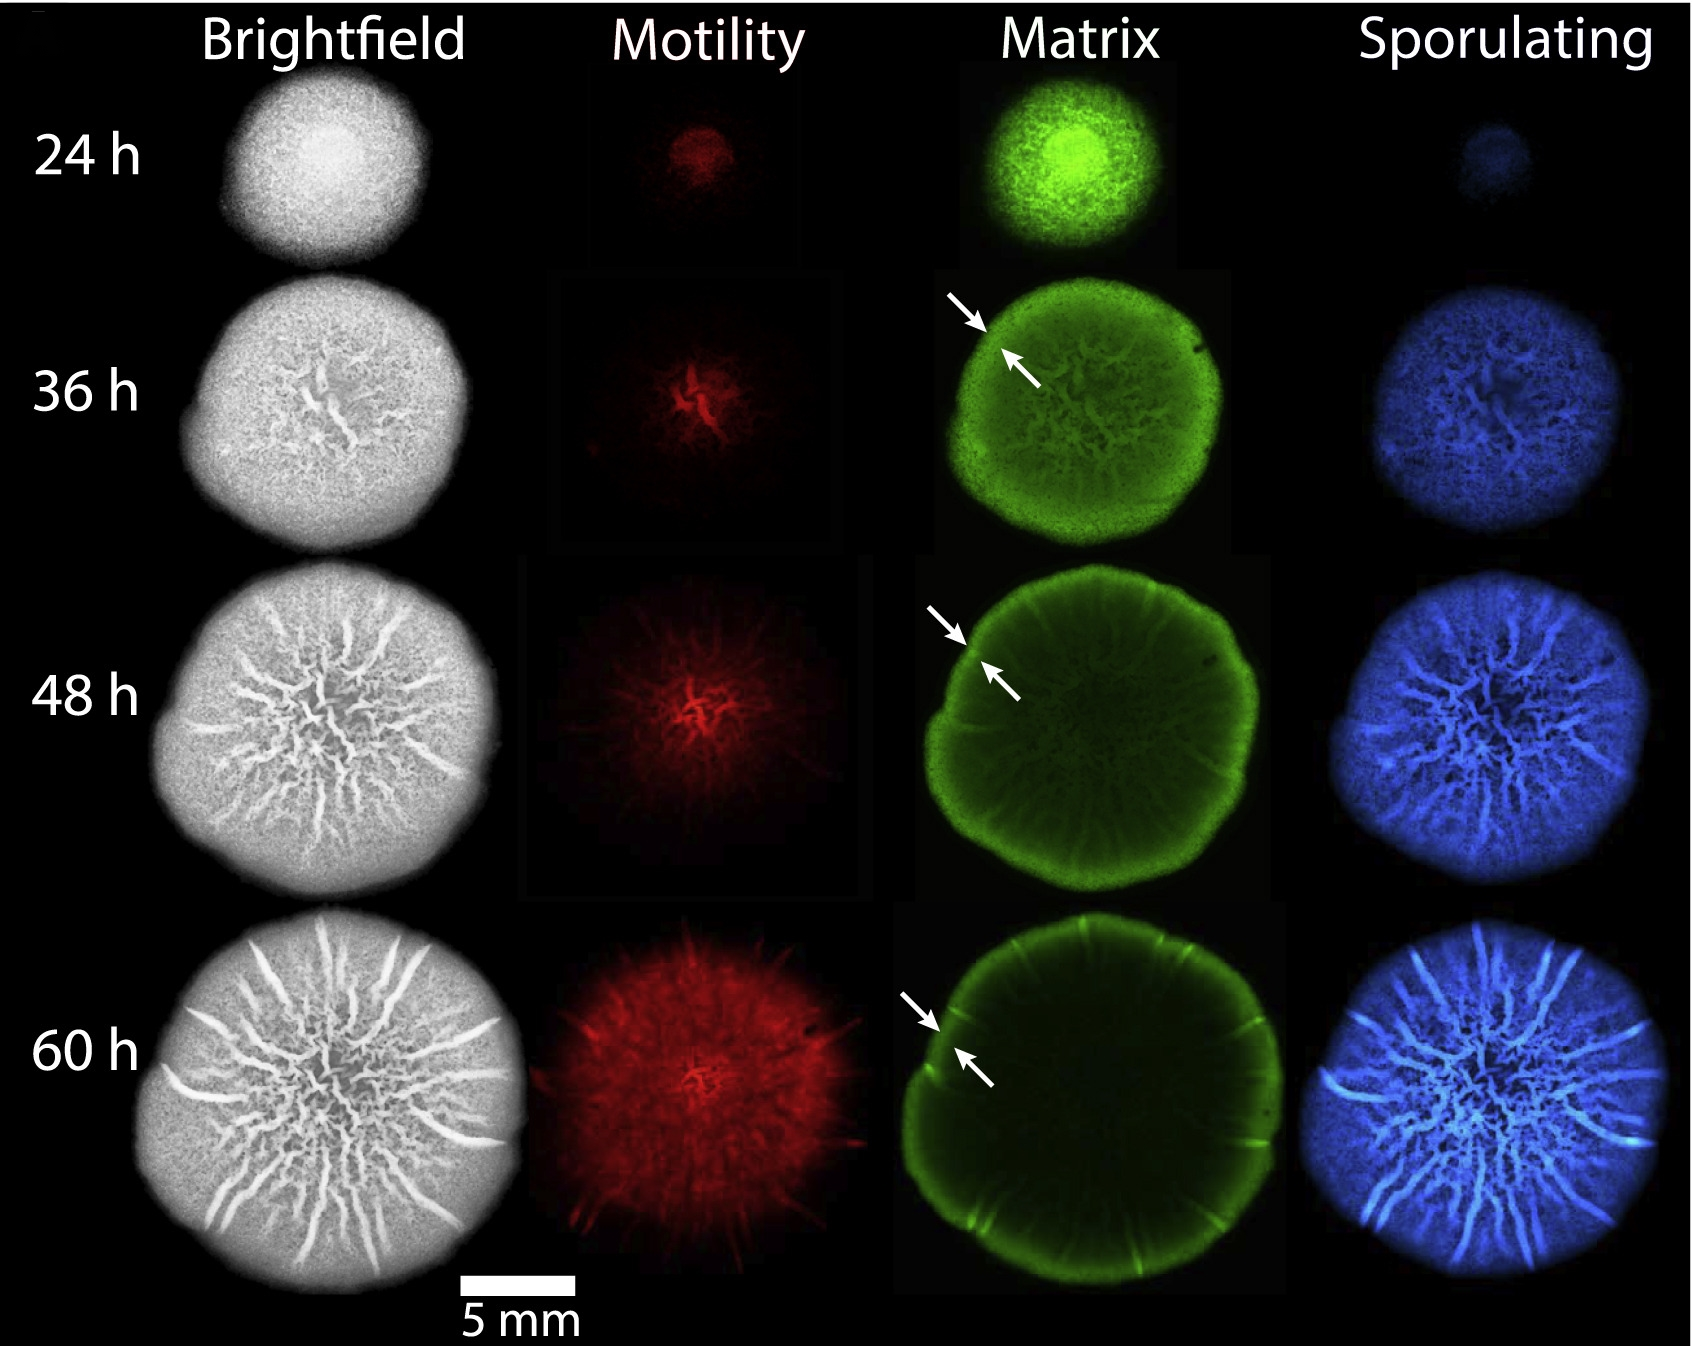
\includegraphics[width=0.8\textwidth]{re}
    \caption{\footnotesize \textbf{Time-lapse of \textit{B. subtilis} biofilm development.} The distinct gene activations are tracked using fluorescent reporters. Activation of genes involved in motility is shown in red, matrix production in green, and sporulation in blue.{\footnotesize\cite{Srinivasan2018}}}


\end{figure}



\section{Paracrine signaling}\label{sec:litrev:theme2}

The observed macroscopic spatial and temporal patterns of gene activation in the \textit{Bacillus subtilis} biofilm suggest a certain level of organization. There is a growing body of evidence suggesting that these patterns are regulated by signaling networks and mechanical interactions between cells, facilitated by signaling molecules that diffuse in the surrounding environment. These communication networks are a common feature of bacterial communities, enabling them to synchronize gene expression. As the density of the cell population increases, these signaling molecules progressively accumulate in the extracellular environment. When reaching a critical concentration, these signaling molecules trigger the coordinated expression of specific genes.{\footnotesize\cite{Arnaouteli2021}}

In many species of bacteria, gene activation and the differentiation of phenotypes are typically regulated by autocrine signaling. Autocrine signaling implies that the cells that produce the signaling molecules are also the same cells that respond to those same signaling molecules. However, in the case of \textit{Bacillus subtilis}, studies suggest that the mechanism of paracrine signaling, rather than autocrine signaling, plays a role in cell differentiation.{\footnotesize\cite{Lpez2009}} This implies that within the biofilm of \textit{B. subtilis}, there is a division of roles among cells. A specific subpopulation specializes in producing a distinct signaling molecule, while another subpopulation responds to this signal. In the case of \textit{Bacillus subtilis}, the ComX pheromone and surfactin are the two most important signaling molecules involved in biofilm formation.{\footnotesize\cite{Chai2011}\cite{Lpez2009}}



\begin{figure}[h]
    \centering
    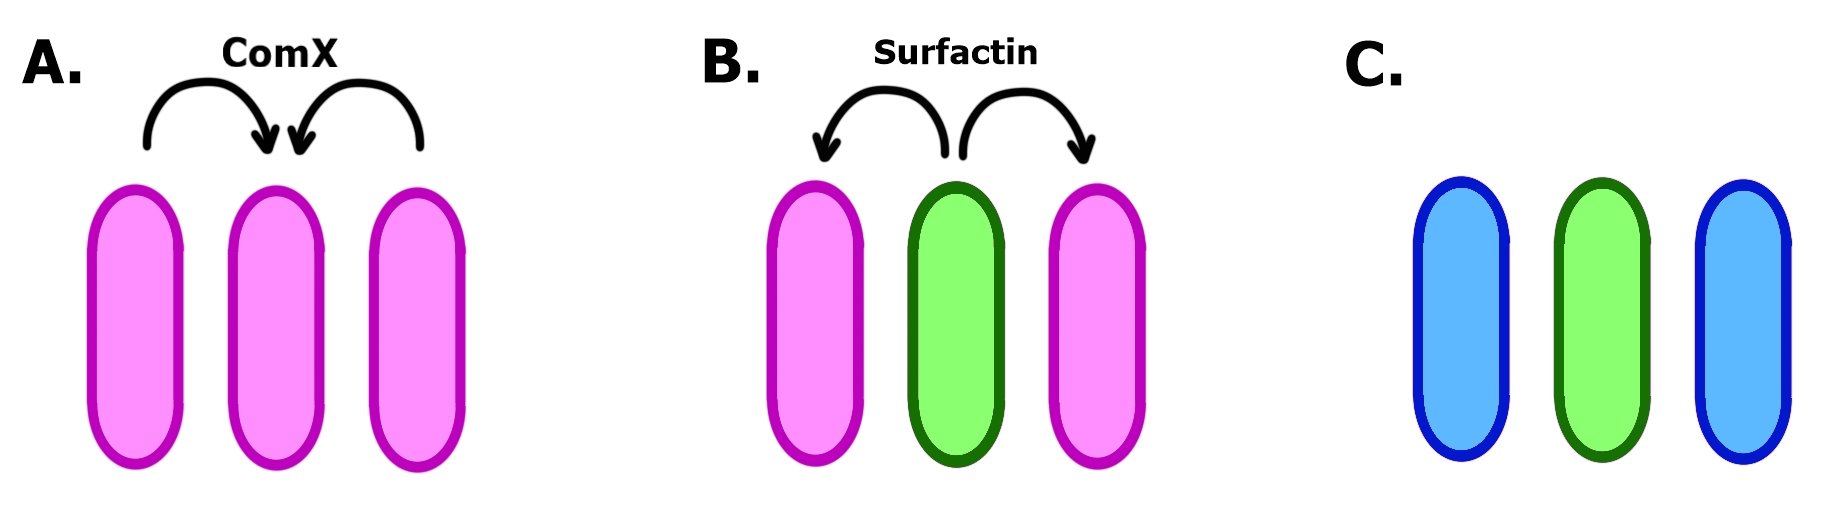
\includegraphics[width=0.8\textwidth]{paracrine}
    \caption{\footnotesize \textbf{Paracrine signaling network in \textit{B. subtilis}} Undifferentiated cells are depicted in pink, surfactin-producing cells are depicted in green, and matrix-producing cells are depicted in blue. A) All undifferentiated cells produce ComX. Some of the undifferentiated cells are particularly sensitive to ComX, which triggers the activation of the surfactin-producing phenotype. B) Surfactin-producing cells secrete surfactin, which affects the neighboring cells. C) Surfactin activates the genes responsible for matrix production in specific, susceptible cells.{\footnotesize\cite{Chai2011}\cite{Lpez2009}}}


\end{figure}
The general overview of the paracrine signaling network in \textit{B. subtilis} is illustrated in Figure 2.2. The ComX molecule is secreted by all bacteria, regardless of their phenotype. As the cell population grows, the concentration of the ComX pheromone accumulates in the extracellular environment until it reaches a higher threshold. Once this threshold is reached, it triggers a subpopulation of nearby bacteria to differentiate into the surfactin-producing phenotype. Then, the subpopulation of bacteria that expresses the surfactin-producing phenotype completely stops growing and reproducing{\footnotesize\cite{Lpez2009}}, and instead begins producing the second signaling molecule: surfactin. Just like ComX, surfactin will begin to accumulate in the environment as the population of surfactin-producing bacteria grows. The high concentration of surfactin in the environment triggers neighboring cells to start producing the extracellular matrix. Interestingly, the cells that produce surfactin are immune to the effects of surfactin. This implies that, as long as a bacterium is expressing the surfactin-producing phenotype, it will not transition into the matrix-producing phenotype. In this sense, the signaling network is a paracrine one.{\footnotesize\cite{Lpez2009}}

Once the bacteria have activated the genes responsible for producing the extracellular matrix, they will develop immunity to the ComX pheromone. This means that the bacteria expressing the matrix-producing phenotype will not switch to the surfactin-producing phenotype. Once again, demonstrating paracrine signaling. The mechanism by which the cell acquires immunity to the ComX pheromone is not fully understood. However, there is evidence suggesting that the extracellular matrix creates a protective layer that inhibits the interaction between ComX and the membrane protein ComP, the protein responsible for sensing ComX.{\footnotesize\cite{Lpez2009}}

\section{Cytoplasmic Gene Regulatory Networks}\label{sec:litrev:theme2}

\subsection{Activation of the surfactin-producing phenotype}\label{sec:litrev:theme2}
The molecular mechanism by which cells switch from one phenotype to another is outlined in Figure 2.3. The ComX pheromone is secreted by all cells and diffuses through the extracellular space. The ComP protein, located in the cell membrane, interacts with the ComX pheromone, which triggers the phosphorylation of the cytoplasmic protein ComA. Upon phosphorylation, ComA is activated and functions as a gene transcription factor for the \textit{srfA} operon. This operon comprises four open reading frames (ORFs) that collectively produce the enzyme surfactin synthetase. Surfactin synthetase is a nonribosomal peptide synthetase, an enzyme that synthesizes peptides such as surfactin without the need for ribosomes. {\footnotesize\cite{Lpez2009}\cite{Rahman2021}}


\begin{figure}[h]
    \centering
    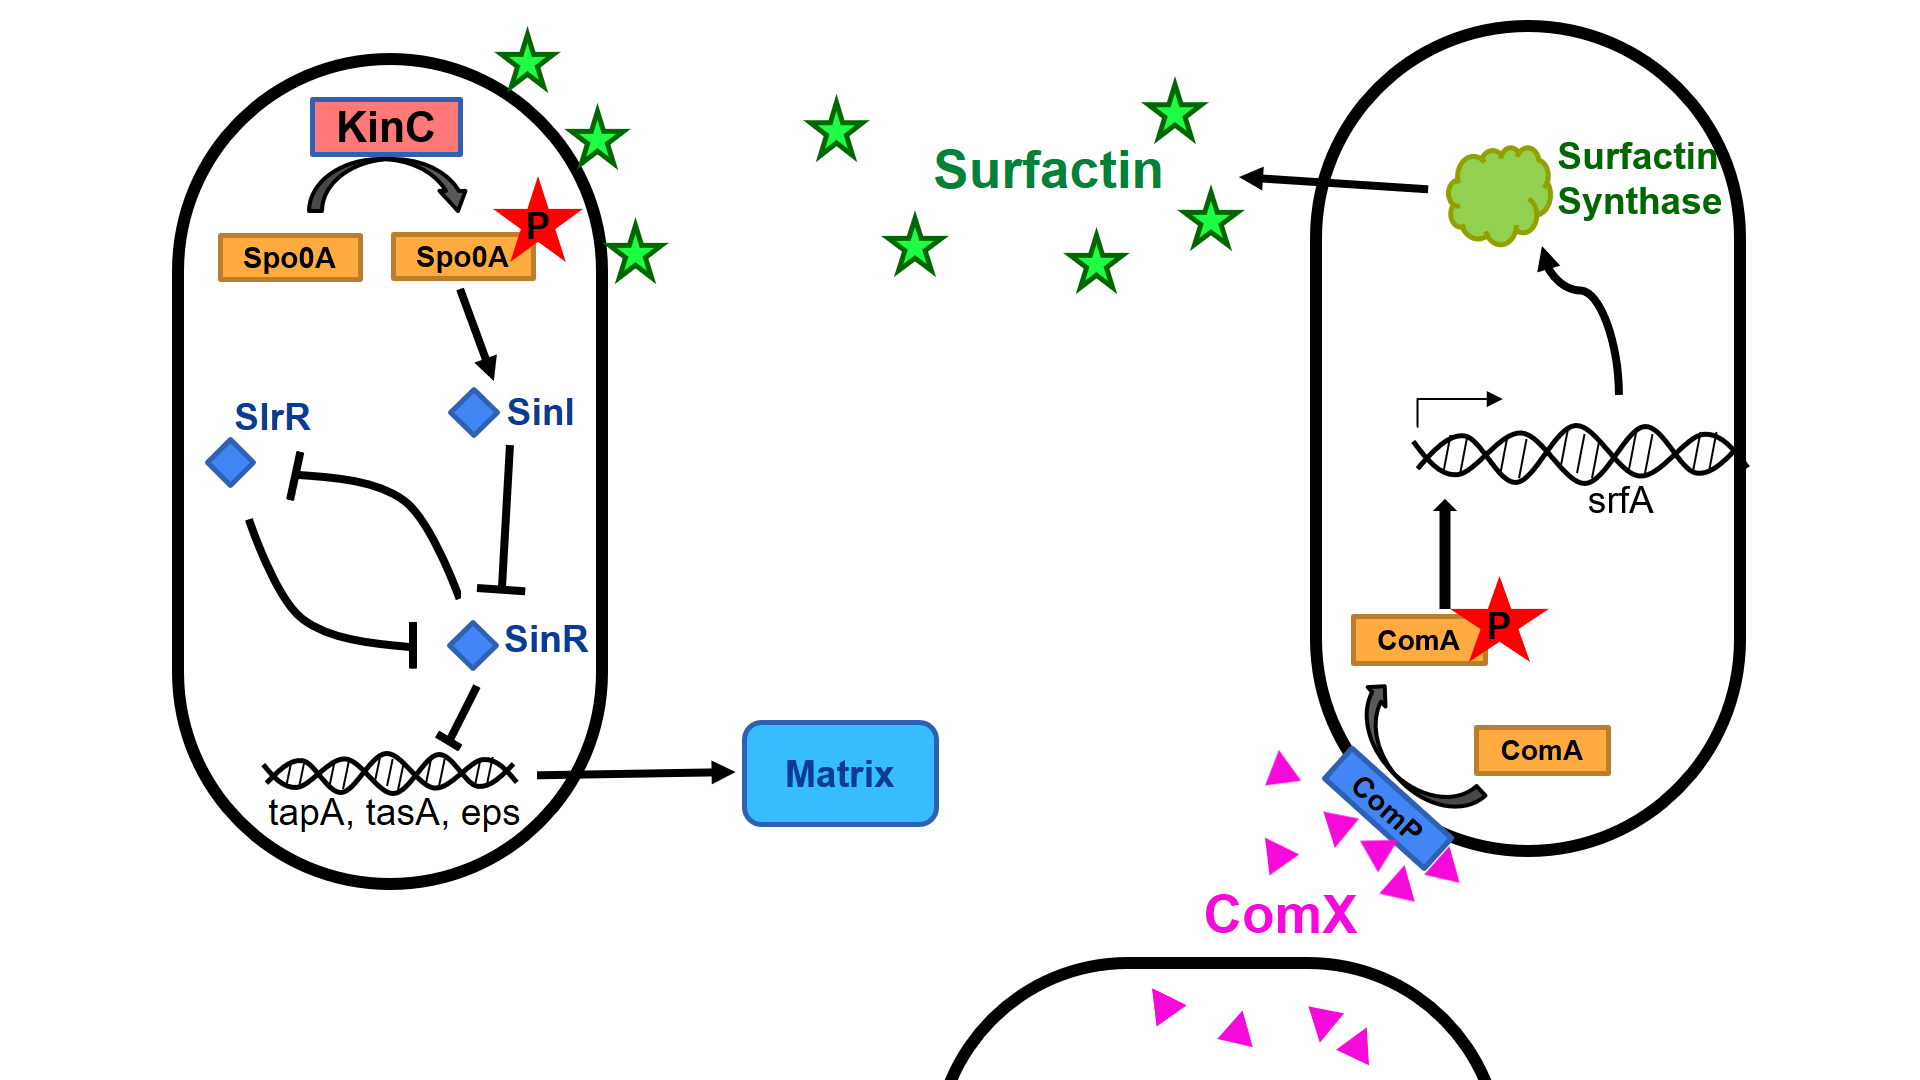
\includegraphics[width=1\textwidth]{Screenshot}
    \caption{\footnotesize \textbf{Extracellular signaling network and cytoplasmatic gene regulatory network} {\footnotesize\cite{Rahman2021}}}



\end{figure}

\subsection{Activation of the Matrix-producing phenotype}\label{sec:litrev:theme2}

Surfactin is known to indirectly activate the expression of genes that produce matrix, although the precise molecular process is not fully understood. It has been suggested that surfactin creates pores in the membrane, leading to the leakage of potassium ions from the cytoplasm to the outside of the cell. This causes the activation of the membrane sensor kinase KinC when potassium levels are low, which then phosphorylates the master gene regulator Spo0A.{\footnotesize\cite{Lpez20091}} However, some studies contradict this exact mechanism.{\footnotesize\cite{Devi2015}}

When Spo0A is activated, it triggers the transcription of the SinI protein. The SinI protein binds to the SinR protein to form a SinI-SinR complex, which effectively titrates SinR, reducing the number of freely available SinR proteins. SinR is a protein that suppresses the transcription of genes related to matrix production. By disabling SinR through the formation of the SinI-SinR complex, the cell can activate the genes responsible for matrix production.{\footnotesize\cite{Chai2011}}

Furthermore, SinR also inhibits the expression of another protein known as SlrR. If SlrR is expressed, it can also suppress SinR by interacting with it to form a SlrR-SinR complex.{\footnotesize\cite{Chai2011}}

\subsection{Mathematical modelling of SlrR-SinI-SinR gene regulatory network}\label{sec:litrev:theme2}
Several authors have formulated systems of differential equations to quantitatively model the biomolecular dynamics involved in the gene regulatory network that controls the expression of the extracellular matrix. The systems of equations describe the changes in the concentration of SinR, SinI, and SlrR proteins in the cytoplasm of individual \textit{Bacillus subtilis} cells over time.{\footnotesize\cite{simon}\cite{Voigt2005}\cite{Newman2013}\cite{Chen2023}\cite{Pedreira2021}\cite{Hallinan2010}}. Having considered the models proposed by these authors, we have decided to adopt a modified version of the model proposed by Dannenberg et al. {\footnotesize\cite{simon}} as the basis for our own model. The model is described by the following system of differential equations:

\begin{align}
\frac{dR}{dt} &= P_{3} - D_{R} R - K_{on(RI)} R I - K_{on(RL)}RL , \label{eq:1} \\
\frac{dI}{dt} &= P_{1}g(R)f(A) - D_{I} I - K_{on(RI)} R I , \label{eq:2} \\
\frac{dL}{dt} &= P_{L}g(R) - D_{L} L - K_{on(RL)} RL, \label{eq:3}
\end{align}

where \(P_3\), \(P_1\), and \(P_L\) represent the maximum production rates of SinR, SinI, and SlrR, respectively. \(R\), \(I\), and \(L\) represent the respective total protein concentrations within a single bacterial cell. \(K_{on(XY)}\) represents the rate constant for the formation of the $(XY)$ complex, while \(D_Z\) encompasses both the dilution rate of component $Z$ caused by cell growth and the degradation rate caused by protein breakdown. The phenomenological activation Hill function \(f(A)\) and the repression Hill function \(g(R)\) are defined as follows:


\begin{align*}
    f(A) &= \left(\frac{(A/K_A)^{n_A}}{1 + (A/K_A)^{n_A}}\right) \\
    g(R) &= \left(\frac{1}{1 + (R/K_R)^{n_R}}\right) \\
\end{align*}  

where $A$ represents the concentration of Spo0A in the cytoplasm. \(K_{A}\) and \(K_R\) represent the binding affinities of Spo0A and SinR, respectively, while \(n_A\) and \(n_R\) represent the cooperativities of the binding.

Equation (\ref{eq:1}) describes the dynamics of the SinR protein concentration in the cell. SinR is produced at a constant rate $P_3$, but its concentration is reduced by a combination of degradation and dilution at a rate $D_R$ due to cell growth. Additionally, the concentration of SinR is affected by its interaction with SinI and SlrR, which form complexes with SinR at rates $K_{on(RI)}$ and $K_{on(RL)}$, respectively, leading to a reduction in free SinR molecules.

Equation (\ref{eq:2}) represents the changes in the concentration of SinI. SinI is produced according to its own maximum production rate $P_1$, which is modulated by the function $g(R)$ that models SinR's repression, and the function $f(A)$ which accounts for activation by Spo0A. Just like SinR, the concentration of SinI is decreased both by degradation and dilution at a rate of $D_I$, and by its binding to SinR, forming the RI complex at a rate of $K_{on(RI)}$.

Lastly, Equation (\ref{eq:3}) represents the dynamics of the SlrR protein concentration. The synthesis of SlrR is again dependant on a production rate ($P_L$), modulated by the function $g(R)$ representing the repressive effect of SinR on SlrR transcription. Similarly, it also considers SlrR's degradation and dilution through the rate $D_L$ and its interaction with SinR, which sequesters SlrR into the RL complex at the rate $K_{on(RL)}$.

The Hill functions in the model represent the regulatory effects of two proteins, Spo0A and SinR, in a phenomenological manner. The activation Hill function \( f(A) \) models the phenomenon in which Spo0A promotes the gene responsible for producing SinI after reaching a critical concentration threshold ($K_A$). This effect exhibits a cooperative nature, meaning Spo0A molecules support each other's binding, resulting in a "switch-like" type of gene activation. On the other hand, the repression Hill function \( g(R) \) describes how SinR inhibits the expression of genes that produce SlrR and SinI. As the concentration of SinR increases above a threshold ($K_R$), the level of repression becomes significant. The Hill functions mathematically represent the biological processes of gene activation and repression in a sigmoidal, threshold-dependent manner.

The system of differential equations just presented is largely similar to the one proposed by Dannenberg et al. {\footnotesize\cite{simon}}. The main difference is that, unlike Dannenberg et al., this thesis will consider the inhibitory effect of SinR on SinI transcription. This inhibitory effect has been proposed and taken into account by other authors {\footnotesize\cite{Voigt2005}\cite{Pedreira2021}\cite{Dundee2022}\cite{Hallinan2010}}

\section{Conclusion}\label{sec:litrev:conclusion}

Drawing from our literature review on \textit{Bacillus subtilis} biofilms and their cellular dynamics, we are set to construct an agent-based model. This model will simulate the complex behaviors of \textit{B. subtilis} cells, integrating the diffusion of extracellular signaling molecules and the gene regulatory networks that control the intracellular concentrations of SinR, SinI, and SlrR. By translating our theoretical insights into a computational framework, we aim to capture the emergent biofilm properties through \textit{in silico} simulation.


% All contribution chapters should follow a similar structure, with a
% mini-introduction and overview at the beginning and a conclusion at the
% end bookmarking a structured presentation of the contribution. This can be
% largely based on your publications.

\chapter{Structure of the Agent-Based Model}\label{chap:contrib1}



The agent-based model of the 2D biofilm monolayer is structured around three main mechanisms. The first mechanism involves the release and diffusion of signaling molecules throughout a two-dimensional grid that covers the entire area of the biofilm. The second mechanism consists of biological functions that occur within individual bacterial cells. These functions include cell growth, reproduction, differentiation of phenotypes, and the detection of chemical signals in the environment. The third mechanism focuses on the physical volume exclusion interactions that occur between cells. These three main mechanisms are implemented in a continuous cycle, sequentially, as shown in Figure 3.1.

\begin{figure}[h]
    \centering
    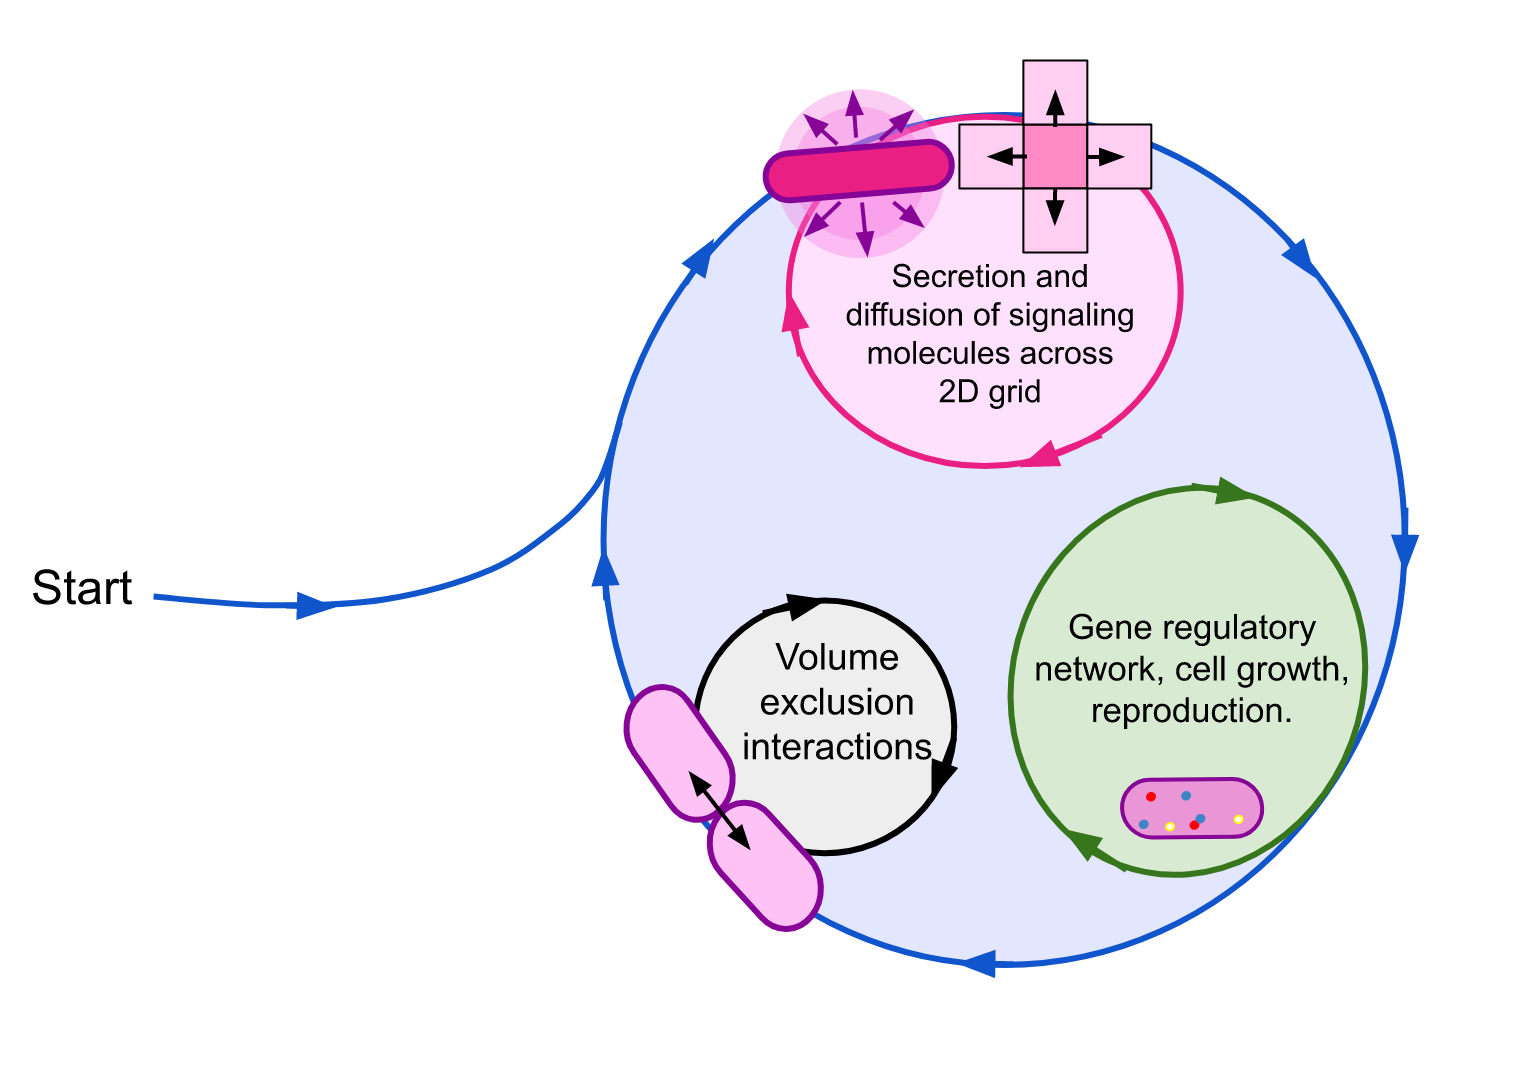
\includegraphics[width=1\textwidth]{cirkl}
    \caption{\footnotesize \textbf{Simulation steps.} The simulation begins with specific initial conditions, such as the starting number of cells, initial phenotypes, initial positions, and initial concentrations of regulatory proteins in the cytoplasm, among others. Then, the simulation runs the main simulation loop, which is subdivided into smaller loops corresponding to the secretion and diffusion of signaling molecules (in pink), biological functions (in green), and volume exclusion interactions (in gray).}

\end{figure} 

\begin{figure}[h]
    \centering
    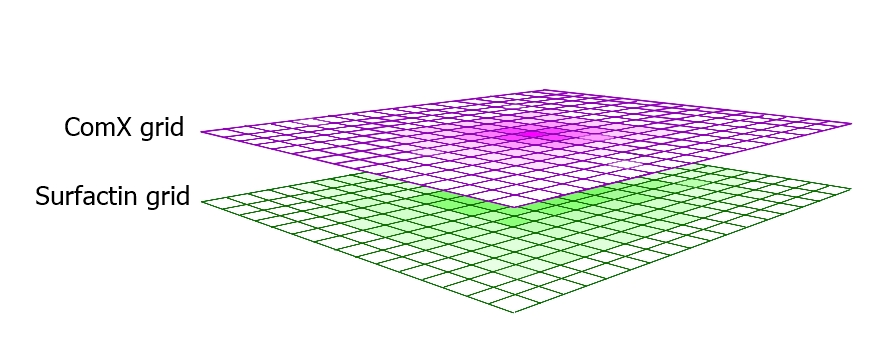
\includegraphics[width=1\textwidth]{grid}
    \caption{\footnotesize \textbf{Grids for numerical simulation of diffusion of signaling molecules}. There is a grid for each relevant substance in the model. The numerical simulation of diffusion runs independently on each separate grid.}

\end{figure}

\section{Secretion and diffusion of signaling molecules on the 2D grid}\label{sec:contrib1:theme1}

The model represents the extracellular environment as a square grid composed of 2025 pixels (45 by 45 pixels), where signaling molecules diffuse. This grid is useful for solving the diffusion equation using the finite difference method. Each pixel represents an area of 10 µm x 10 µm. The columns and rows of the grid define the coordinates of the two-dimensional space. In this space, each pixel represents the concentration of a signaling molecule at a specific coordinate. The model aims to simulate the diffusion process of two substances: ComX and surfactin. It employs separate, independent grids for each substance, as illustrated in Figure 3.2.

Every bacterium has the ability to interact with the pixel grid, either by secreting a substance onto the grid or by sensing it. In each iteration of the simulation, bacteria release a small amount of signaling molecules into the nearest pixel. Immediately after this release, the simulation performs a diffusion step to smooth out the initial peak resulting from the release of the signaling molecules. The detailed mathematical aspects of the diffusion simulation are presented in Chapter 4.




\section{Biological functions}\label{sec:contrib1:theme1:A}

The bacteria have been programmed to perform the following biological functions:

\subsection{Motion} This function introduces a small random force and torque to each individual bacterium, simulating Brownian motion. The random motion and growth of bacteria often result in bacterial cells overlapping in volume. A volume exclusion mechanism, which will be explained later, resolves this overlap.

\subsection{Growth} This function multiplies the length of each individual bacterium by a specific scaling factor greater than 1. To prevent large groups of bacteria from duplicating simultaneously, the growth rate and reproduction length are varied throughout the simulation by adding a small random value to these parameters for each individual bacterium. In this way, we prevent synchronized reproduction.


\begin{figure}[h]
    \centering
    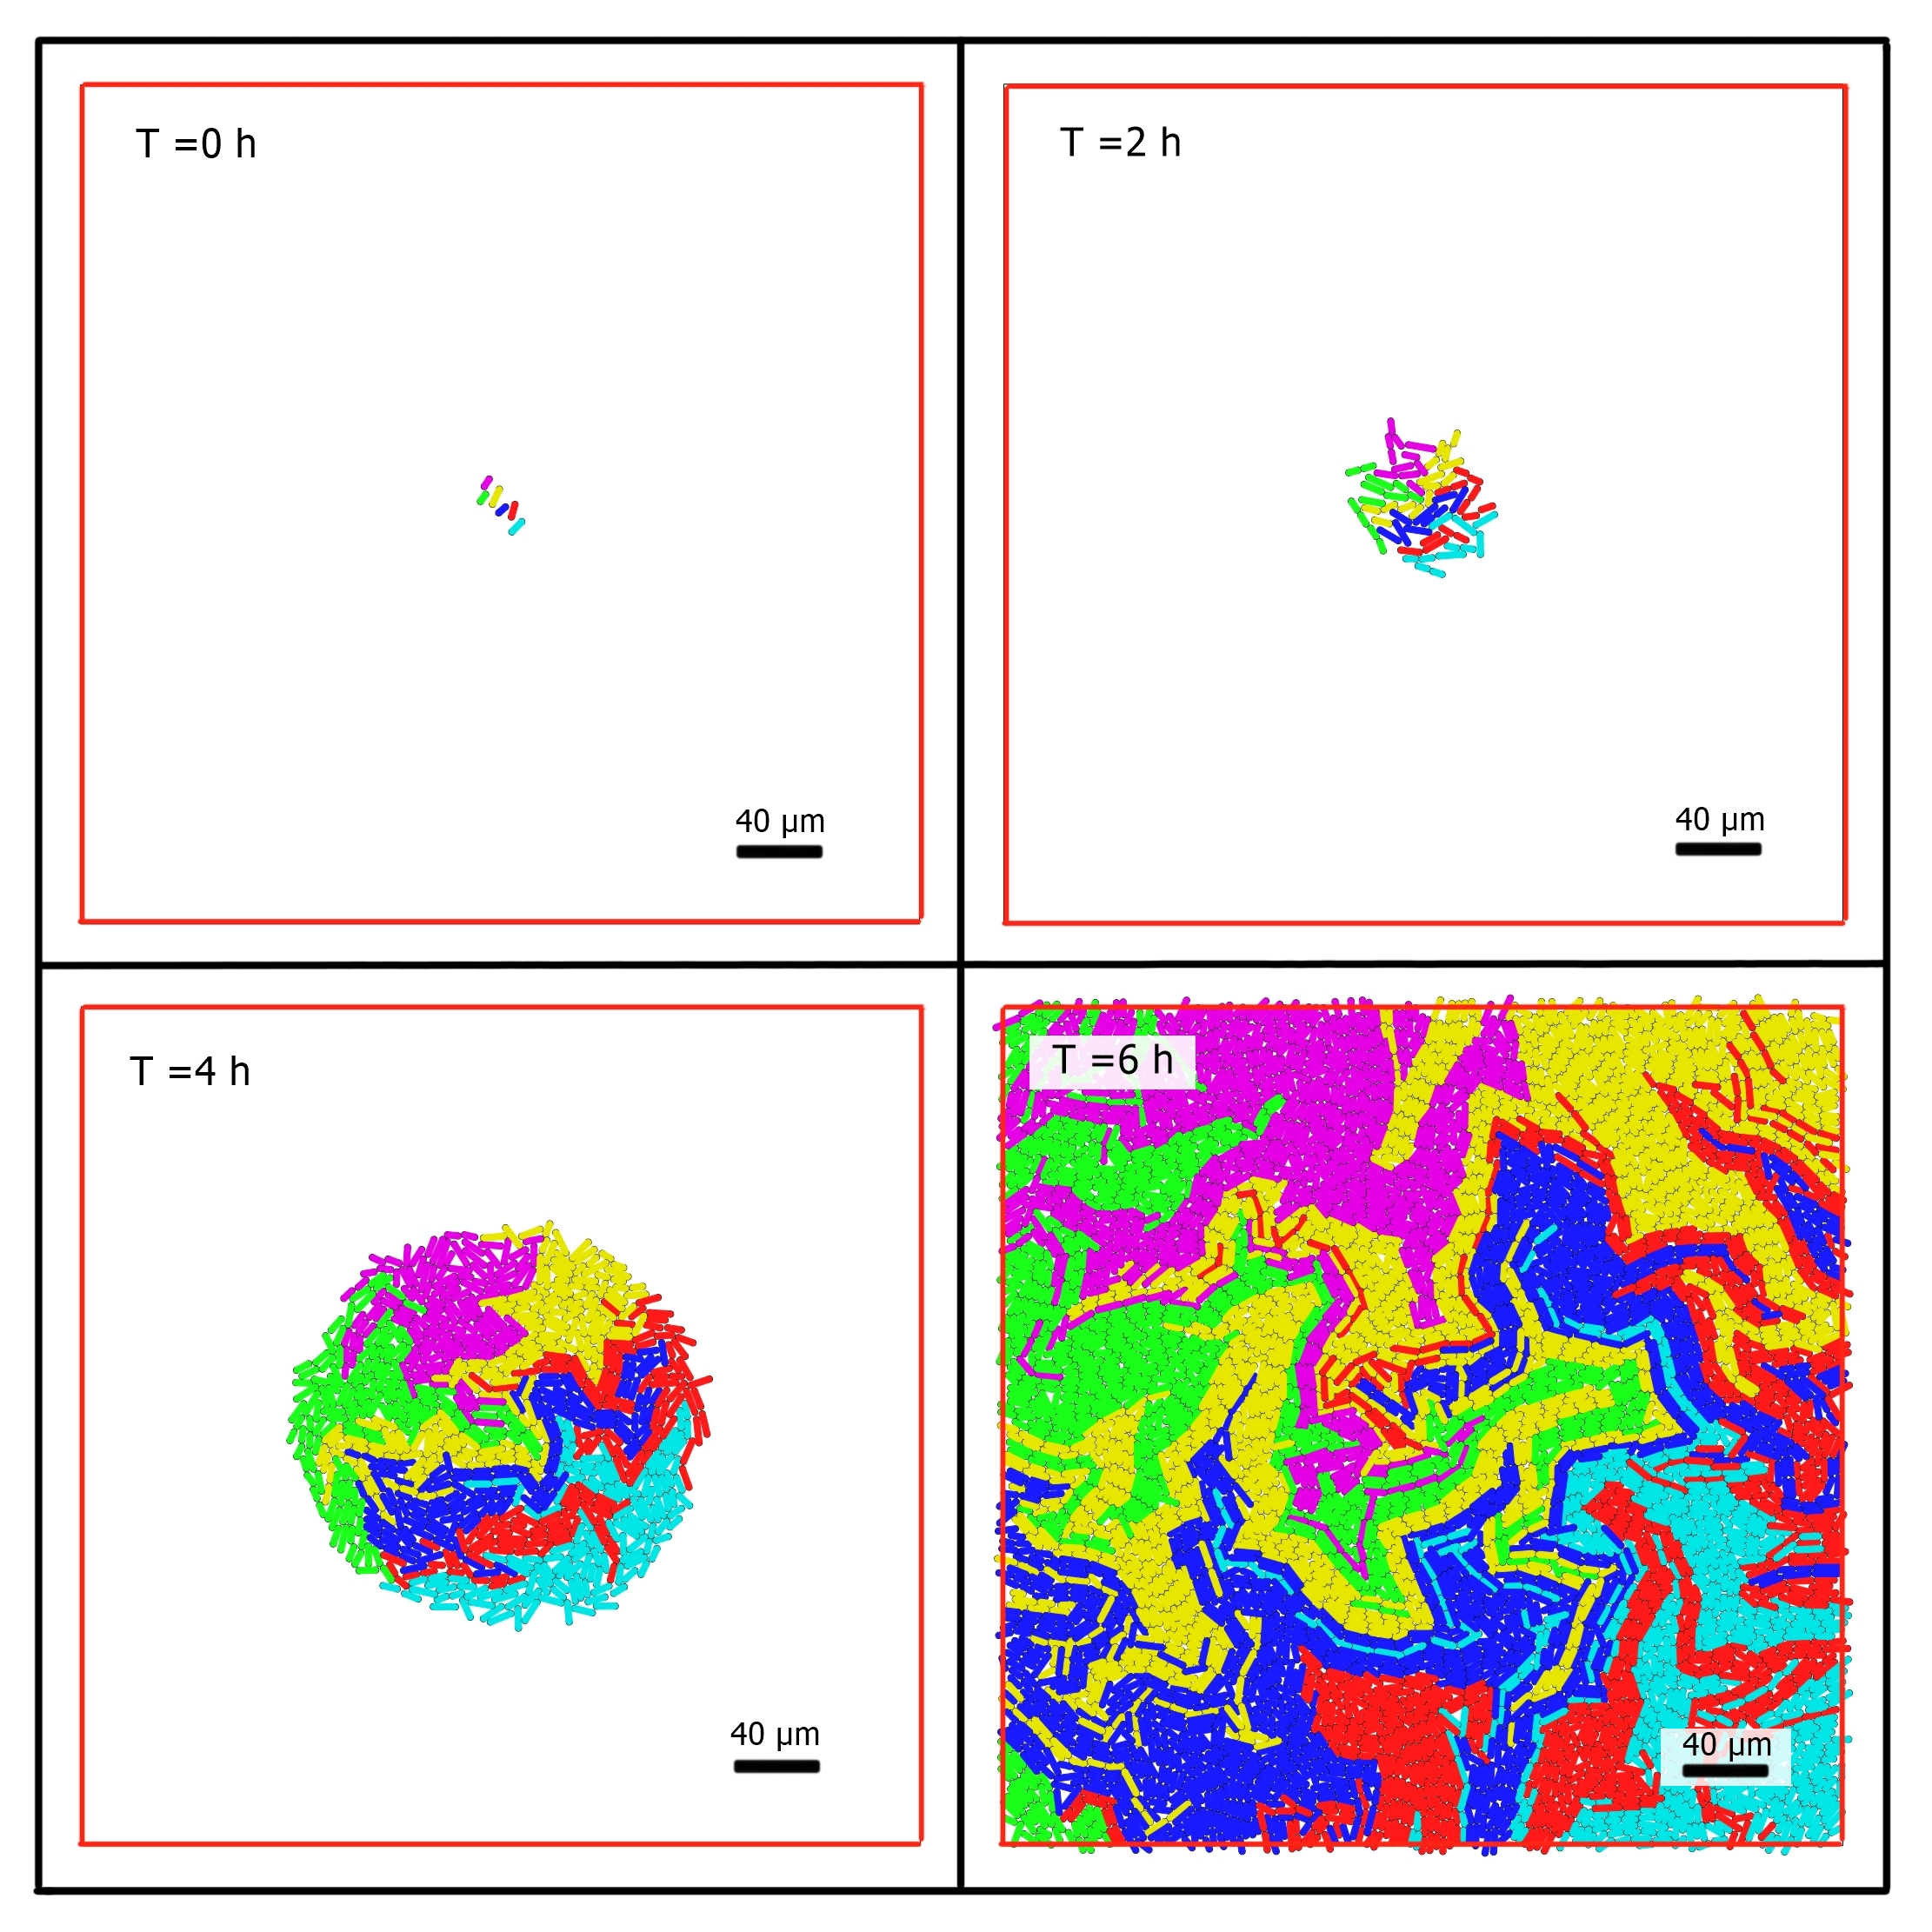
\includegraphics[width=0.9\textwidth]{New_engine2.jpg}
    \caption{\footnotesize \textbf{Demonstration of cell growth, reproduction, and inheritance.} The top-left corner shows six bacteria at the initial time step. Each of the six colors represent a distinct cell lineage. The top-right, bottom-left, and bottom-right panels show the color-coded offspring of the initial bacteria after 2, 4, and 6 hours, respectively. The red square represents the simulation area, which measures 0.16 mm\(^2\), where the bacteria are allowed to exist. If the bacteria escape from this area, they will be removed from the simulation}
\end{figure}
\subsection{Reproduction and Inheritance} When a bacterium's length reaches a certain threshold for reproduction, this function generates a new offspring bacterium adjacent to the parent bacterium. Some properties of this offspring bacterium, such as the cytoplasmic concentration of regulatory proteins, are inherited from the parent, while others, such as the threshold for reproduction length and sensitivity to signaling molecules, are randomly determined at birth. The ability to pass on traits from parents to their offspring allows us to visually track the offspring of each bacterium by assigning a color to the bacterium as an inheritable characteristic, as shown in Figure 3.3.


\subsection{Gene Regulatory Network} This function performs one iteration of the system of differential equations that represents the Gene Regulatory Network described in Section 2.4.3. It models the changing cytoplasmic protein concentrations of SinR, SlrR, and SinI within each individual bacterium. The fact that the network is simulated independently within each bacterium's cytoplasm means that at any given simulation step with $N$ bacteria, there are $N$ independent instances of this system of differential equations being solved simultaneously and decoupled from each other.

\subsection{Phenotype Differentiation} This function determines whether the conditions are suitable for gene expression or phenotype transition. For instance, if the concentration of ComX exceeds a certain stochastic threshold, the bacteria will transition into the surfactin-producing phenotype. If the internal concentration of the regulatory protein SinR falls below a certain stochastic threshold, the bacteria will transition into the phenotype that produces the extracellular matrix.

In this model, each bacterial cell has a unique sensitivity threshold to the concentration of extracellular ComX and cytoplasmic SinR. The sensitivity to ComX is a uniformly distributed random variable between 50 and 150 Arbitrary Units (AU), and it remains constant over time for individual bacteria. This means that, on average, half of the undifferentiated cells will transition to the surfactin-producing phenotype once they detect an extracellular concentration of ComX of 100 (AU) or higher. According to this model, sensitivity to ComX is a population trait that is not inherited from the parent bacteria. Instead, it is randomly determined at the moment of birth. The stochasticity of this trait within the population is the reason why it may appear that certain bacteria are sensitive to ComX, while others are not. In this way, a sufficiently high concentration of ComX will trigger any undifferentiated bacteria to become surfactin-producing bacteria. However, for a few bacteria, the stochastic threshold is so high that it will never be reached under normal conditions of cell density, ComX diffusion constant, and ComX production rate.

In the pathway involving surfactin, Spo0A, and KinC, we had to make some assumptions to simplify the model. We defined the intracellular concentration of Spo0A to be a linear function of the extracellular concentration of surfactin. This decision was based on the rough estimation of the presumed cytoplasmic concentration of Spo0A and the suggested molecular mechanism of Spo0A activation by surfactin through KinC phosphorylation (as illustrated in Figure 2.3). However, the interaction between these molecules could be further explored to develop a more comprehensive and detailed model.

Regarding the system of differential equations described in Section 2.4.3, we defined the SinR sensitivity threshold as a uniformly distributed random variable ranging from 47.5 to 52.5 nM. This means that, on average, half of the undifferentiated cells will transition to the matrix-producing phenotype once they detect a concentration of SinR that is 50 nM or lower.

\section{Volume exclusion interactions}\label{sec:contrib1:theme2}

The open-source TypeScript library, Box2d.ts, handles volume exclusion interactions, motion, and bacteria positions in the simulation. This 2D physics library helps to create animations that simulate the movements and interactions of rigid 2D objects. It offers tools for simulating physical phenomena like gravity, collisions, air resistance, and other forces that are specific to 2D graphics.{\footnotesize\cite{Catto2023}} For more information, please refer to section 7.1.

Without the volume exclusion mechanism, the growth and division of bacteria could result in overlapping cell volumes. The volume exclusion mechanism ensures that cells are displaced during their growth and division, as shown in Figure 3.3.

Additionally, this library was utilized to control the maximum number of bacteria allowed to coexist simultaneously within the simulation area. This control mechanism is crucial because unregulated bacterial exponential growth would make the simulation unmanageable. To achieve population control, there is a designated area of 0.16 mm\(^2\) within the simulation where the bacteria are allowed to exist. If a bacterium is pushed outside this area by its growing siblings, it will be eliminated from the simulation. According to our simulations, the maximum allowable amount of bacteria in this 0.16 mm\(^2\) area is approximately 5200 cells.


\section{Conclusion}\label{sec:contrib1:conclusion}

% Here we will summarize the contribution, and describe a logic transition to the next chapter.

%In this chapter, we presented the overall structure of the agent-based model of the 2D biofilm monolayer, which consists of three main mechanisms: the secretion and diffusion of signaling molecules on the 2D grid, biological functions like growth and reproduction, and volume exclusion interactions. In the following chapter, we will discuss the mathematical principles involved in simulating diffusion on a 2D grid. Additionally, we will also present the calculations used to determine the time scales at which several processes occur in the model.

% Let's make it better. We can do it!

In this chapter, we have presented the basic mechanisms of the agent-based model for the two-dimensional biofilm monolayer. The model consists of three main mechanisms: the secretion and diffusion of signaling molecules on a two-dimensional grid, biological functions such as growth and reproduction, and volume exclusion interactions. In the upcoming chapter, we will discuss the mathematical principles involved in simulating diffusion on a two-dimensional grid. Additionally, we will also present the calculations used to determine the time scales at which several processes occur in the model.


% All contribution chapters should follow a similar structure, with a
% mini-introduction and overview at the beginning and a conclusion at the
% end bookmarking a structured presentation of the contribution. This can be
% largely based on your publications.

\chapter{Dimensional Analysis and Parameters}\label{chap:contrib2}

To validate the dimensions of the parameters in our simulations, we used two key parameters as reference points: the length of the bacteria (as a spatial reference) and the bacterial doubling time (as a temporal reference). The dimensions of the remaining parameters in this simulation, such as the diffusion coefficient, grid size, and reaction rates, were calculated relative to these two parameters.

\section{Spatial and Temporal Points of Reference}\label{sec:contrib2:theme1}

\subsection{Bacterial Length}\label{sec:contrib2:theme1:A}

In the context of a typical \textit{Bacillus subtilis} cell, which measures approximately 6 µm in length, we defined the reproductive length as a random variable with a uniform distribution between 12 and 12.1 µm. Consequently, the maximum length that a bacterial cell can reach is approximately 12 µm just before binary fission, while the minimum length is about 6 µm immediately after binary fission.

\subsection{Bacterial Doubling Time}\label{sec:contrib2:theme1:B}

The growth rate per simulation time step is defined as a dimensionless random variable uniformly distributed between 1.002 and 1.003. The range of this random variable was intentionally chosen to ensure that the physics engine library can accurately compute the volume exclusion forces at each simulation time step without any unresolved overlaps. A higher growth rate would lead to rapid cell growth, causing excessive overlap in volume between the bodies of the bacteria. If the overlap is too large, it may not be fully resolved by the physics engine within a single simulation time step. The random fluctuation in the growth rate causes the size of bacteria, on average, to increase by a factor of 1.0025 at each time step.

While it might have been possible to calculate the exact doubling time analytically by assuming a constant growth rate, constant reproductive length across the population, and assuming that bacterial bodies are perfectly rectangular (as opposed to rods with rounded ends), we chose to estimate the doubling time through numerical simulations. This numerical methodology was chosen as a practical approach to account for the stochastic nature of the bacteria's growth rate and reproductive cycle, as well as the nuance that the length of the bacteria does not exactly represent the distance from one rounded end to the other rounded end of the bacteria.

\begin{figure}[h]
    \centering
    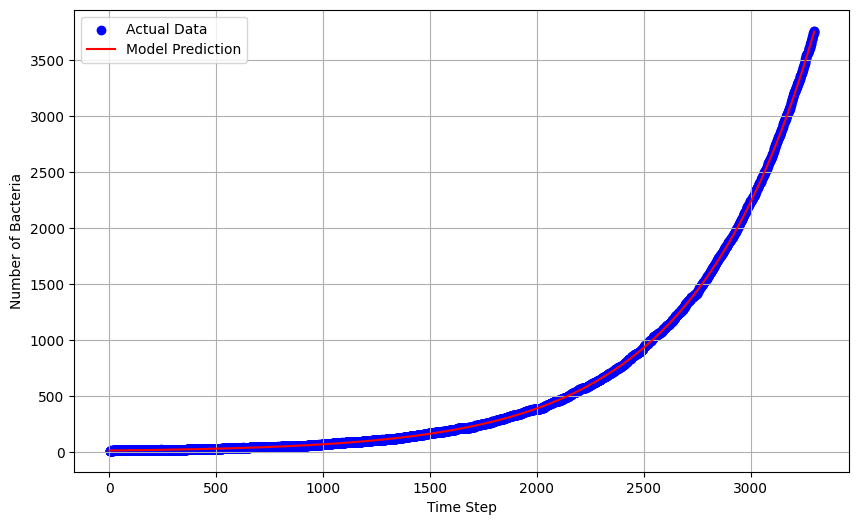
\includegraphics[width=1\textwidth]{Exponential_growth}
    \caption{\footnotesize \textbf{Bacteria cell count over simulation time steps.} The total number of bacteria in the simulation after each time step is shown in blue. The fitted model for exponential growth is shown in red.}

\end{figure}

To calculate the doubling time, we allowed the bacteria to grow and reproduce until the population reached approximately 3700 bacteria, similar to the growth and reproduction progression depicted in Figure 3.3. We recorded the number of bacteria at each time step of the simulation. Figure 4.1 illustrates the cumulative bacterial count during a growth simulation. The bacterial doubling time was determined by fitting a non-linear regression model to the data points obtained from simulations. The exponential growth equation \(y = b \cdot e^{mt}\) is used as a model, where \(y\) represents the cell count at the discrete time step \(t\), \(b\) represents the initial cell count, and \(m\) represents the growth rate.

In the fitted regression model, the parameters \(b\) and \(m\) were estimated to be approximately 11.74 bacteria and 0.00175, respectively. The coefficient of determination $(R^2)$ for this model is approximately 0.9997.

The estimated parameter \(m\) can be used to calculate the doubling time \(\tau\) using the following equation:


\[
    \tau=\frac{{\ln(2)}}{m} 
\]

which results in a doubling time of $\approx$ 396 simulation time steps.


Given that the actual doubling time of \textit{Bacillus subtilis} in optimal conditions is around 30 minutes, we can use the above estimate to set one simulation time step to represent 5 seconds. Taking this into consideration, the calculated doubling time for the simulated bacteria is 33 minutes.





\section{Numerical Simulation of the Diffusion Equation}\label{sec:contrib2:theme2}

The diffusion equation is a partial differential equation that describes the behavior of a substance as it spreads out over time due to random motion. It serves as a fundamental model for understanding heat distribution, particle dispersion, and other processes characterized by the flow from regions of higher concentration to regions of lower concentration. The standard form of the diffusion equation in two dimensions is:

\[
\frac{\partial u}{\partial t} = D \left( \frac{\partial^2 u}{\partial x^2} + \frac{\partial^2 u}{\partial y^2} \right),
\]

where $u$ represents the concentration of the diffusing substance at a given point, $D$ is the diffusion coefficient, and $t$, $x$, and $y$ are the time and spatial variables, respectively. {\footnotesize\cite{caltech}}

To numerically simulate the diffusion equation, we apply the finite difference method, which is a well-established numerical technique for solving partial differential equations. This involves discretizing the spatial domain into a grid and approximating the continuous derivatives with respect to time and space by using the differences between grid point values. We construct a matrix representation of the diffusion field \(u_{n+1}[i,j]\), which represents the concentration of substance \(u\) at each grid position \([i,j]\) and at each time step \(n+1\).

The concentration \(u\) is updated iteratively for each grid position based on the previous time step \(n\) and the influence of its neighboring grid points. This update is governed by the discrete diffusion equation:

\[
u_{n+1}[i][j] = u_{n}[i][j] + \gamma  \left( u_{n}[i+1][j] + u_{n}[i][j+1] + u_{n}[i-1][j] + u_{n}[i][j-1] - 4  u_{n}[i][j] \right)
\]

where \(\gamma\) is a constant given by 

\[ \gamma = D \frac{{\Delta t}}{{(\Delta x)^2}},  \]

with \(D\) being the diffusion coefficient of $u$, \(\Delta t\) representing the time step increment, and \(\Delta x\) signifying the spatial step size or the grid resolution. {\footnotesize\cite{gitconnectedSolvingHeat}\cite{unimuenster}}

To ensure computational stability for this numerical method, it is crucial to satisfy the following condition, which requires the time step \(\Delta t\) to be sufficiently small:

\[\frac{{\Delta t}}{{(\Delta x)^2}} \leq \frac{1}{{4D}}.\]

Fulfilling this criterion ensures the convergence of the solution and helps to avoid numerical oscillations. {\footnotesize\cite{gitconnectedSolvingHeat}\cite{unimuenster}}

For a rough estimate of the diffusion constant \(D\) of signaling molecules in our simulation, we can consider the order of magnitude to be similar to that of glucose diffusing in water, which is roughly 100 \(\mu m^2/s\) {\footnotesize\cite{Bashkatov2003}}. With a specified grid resolution in which each element has an area of 10 \(\mu m\) by 10 \(\mu m\), the stability condition can be used to calculate the maximum allowable time step \(\Delta t\) to solve the diffusion equation, yielding \(t \leq 0.25\) s.

Since the time step for bacterial growth is 5 seconds (as calculated in section 4.1.2), we need to perform the diffusion numerical iterations more frequently than the time step in which the bacteria are growing. This means that for each time-step that the bacteria use to grow, the diffusion equation undergoes 20 time-steps to update the concentration of the extracellular signaling molecules.


\section{Regulatory gene circuit}\label{sec:contrib2:theme2}


The agent-based model simulates the evolution of cytoplasmic concentrations of regulatory proteins by solving the system of differential equations described in Section 2.4.3. The Euler method was used to solve the equations using a time step of 1 minute. This 1-minute time step was determined through a trial-and-error process aimed at finding the largest possible time step that maintains computational efficiency without compromising the stability of the numerical simulation. During the trial-and-error process, we utilized the three-dimensional phase space to track the trajectories of SinR, SinI, and SlrR concentrations over time. The code for visualizing the solutions in phase space is provided in section 7.3.

The magnitude and dimensions of the parameters used to simulate this system of equations are presented in Table 4.1. These parameters are based on the typical rates and thresholds observed in biological systems. However, they are still rough approximations of the exact real values for the case of \textit{B. subtilis}. Most of the parameters shown in Table 4.1 were chosen with reference to the models and estimations presented in ({\footnotesize\cite{simon}\cite{Voigt2005}\cite{Newman2013}\cite{Chen2023}\cite{Pedreira2021}\cite{Hallinan2010}}).

Two parameters, \(K_A\) and \(K_R\), were defined as uniformly distributed variables across the population to introduce stochasticity into the system of differential equations. The reason for introducing this slight stochasticity into these two parameters is that we do not expect real bacteria to have identical effective reaction rates with every other bacterium. In reality, we assumed that the effective reaction rates vary across the population due to diverse cytoplasmic conditions unique to each bacterium, including other inhibitors and activators not accounted for in this model, such as SlrA and AbrB. The parameters were fine-tuned by observing the behavior of the solution trajectories in phase space and ensuring that they replicated the expected switch-like behavior previously documented in the literature. In any case, the parameters were kept within typical values for biological systems.

  \begin{table}
    \centering
    \caption{\footnotesize Parameters for SinR-SlrR-SinI gene regulatory network}
    \label{table:parameters}
    \begin{tabular}{|c|c|c|}
      \hline
      Parameter & Value & Units  \\
      \hline
      \(P_3\) & 1.5 & nM/minute \\
      \(P_1\) & 1.5 & nM/minute \\
      \(P_L\) & 1.25 & nM/minute \\
      
      \(D_R\) & 1.4 \(\times 10^{-2}\) & 1/minute  \\   
      \(D_I\) & 1.4 \(\times 10^{-2}\) & 1/minute  \\
      \(D_L\) & 1.4 \(\times 10^{-2}\) & 1/minute  \\ 
      \(K_{on(RL)}\) & 1 \(\times 10^{-3}\) & 1/(minute\(\cdot\)nM)  \\
      \(K_{on(RI)}\) & 1 \(\times 10^{-3}\) & 1/(minute\(\cdot\)nM)  \\ 

      
      \(K_A\) & \( \sim U(47.5, 52.5)\) & nM  \\
      \(K_R\) & \( \sim U(52.5, 57.5)\) & nM \\

      

      \(n_A\) & 4 & -  \\
      
      \(n_R\) & 4 & -  \\
    
      \hline
    \end{tabular}
  \end{table}
  \section{Secretion of Signaling Molecules}\label{sec:contrib2:theme2}
  Our understanding of the exact rates at which ComX and surfactin are produced and degraded during the various stages of \textit{B. subtilis} biofilm development is still incomplete. Similarly, the exact concentrations of surfactin, ComX, and SinR that induce a phenotype transition are not completely clear. To address this, we have designed our agent-based model to represent the concentrations of ComX and surfactin in arbitrary units (AU). Future studies could then adjust these dimensionless concentrations using experimental parameters obtained from real-world data.
  
  We have designed the simulation so that every 0.25 seconds (the same time step as for solving the diffusion equation), every single bacterium secretes a small fixed amount of ComX, regardless of the cell's specific phenotype. In addition to the ComX that every bacterium secretes, bacteria belonging to the surfactin-producing phenotype also secrete an additional fixed amount of surfactin at the same time step. This means that surfactin producers secrete two signaling molecules: ComX and surfactin. Non-surfactin producers will only produce ComX. The reason why every bacterium in our simulation produces ComX is that we assumed that the \textit{comX} gene is constitutively expressed.

  Given that the number of surfactin producers is significantly smaller than the number of ComX producers, we set the surfactin production to be ten times that of the ComX production. This makes it easier to visualize and compare the concentration of both substances during the simulation.

  \section{Conclusion}

  Having established the mathematical methods and the arguments for the parameters and assumptions used in the simulation, we can now proceed to the simulation results. The results will be presented in the following chapter.
    
  
  

 
% All contribution chapters should follow a similar structure, with a
% mini-introduction and overview at the beginning and a conclusion at the
% end bookmarking a structured presentation of the contribution. This can be
% largely based on your publications.

\chapter{Simulation of Biofilm Development}\label{chap:contrib3}

\section{Progression of a Simulated Biofilm Monolayer}

We present the sequential development of a simulated biofilm monolayer. We will analyze the evolution of the cytoplasmic proteins involved in the gene regulatory network and the development of phenotypes at 1-hour intervals, starting from the 4th hour after inoculation.

\subsection{After 4 Hours}\label{sec:contrib3:theme1}

During the first 4 hours of the simulation, the initial cells, commonly known as pioneer cells, initiate the process of biofilm formation. This group of cells consists exclusively of undifferentiated cells (Figure 5.1). The initial group of cells secretes the ComX pheromone, which rapidly diffuses across the grid of pixels in all directions. According to our model, each bacterium produces the ComX pheromone constitutively, regardless of its phenotype or environmental conditions. The continuous production of the ComX pheromone makes it an effective indicator of cell density. At this stage of biofilm development, no cells express the surfactin-producing phenotype, resulting in a complete absence of surfactin in the extracellular space.

At this point, the concentration of SinR molecules in every cell exceeds 75 nM. This is due to the absence of SinI or SlrR molecules for binding, and the production rate of SinR \(P_3\) is greater than the dilution rate caused by cell growth and degradation \(D_{R}\). Conversely, the concentration of SinI and SlrR is very low. The absence of SinI molecules at this stage is due to the absence of surfactin in the environment, which is necessary to stimulate SinI transcription. The absence of SlrR molecules is due to the high concentration of SinR, which strongly inhibits the expression of SlrR.

\begin{figure}[h]
    \centering
    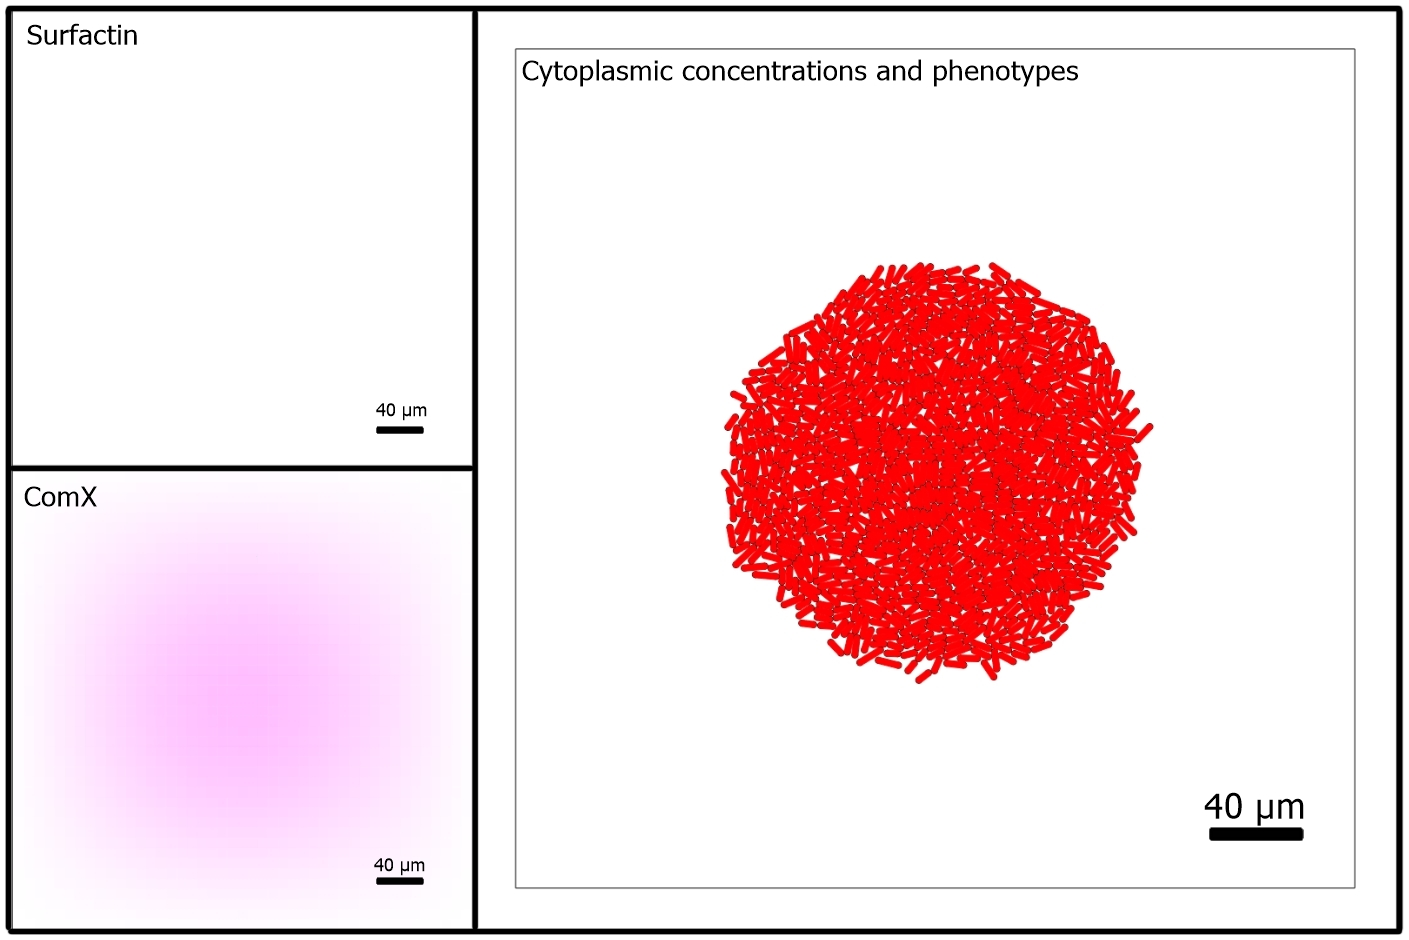
\includegraphics[width=0.98\textwidth]{Final_run4.jpg}
    \caption{\footnotesize \textbf{Extracellular and intracellular concentrations of signaling molecules and gene regulatory proteins 4 hours after inoculation.} The image in the top-left corner shows the extracellular concentration of surfactin across the biofilm, which, at this stage of development, is zero. The image in the bottom left corner shows the extracellular concentration of ComX across the biofilm, measured in arbitrary units. The intracellular concentrations of SinR, SinI, and SlrR are represented as a point in the three-dimensional red-green-blue additive color space. Specifically, SinR concentration is mapped to the red channel, SinI to the green channel, and SlrR to the blue channel. Since all cells have a high concentration of SinR and a low concentration of SinI and SlrR, they all appear 100\% red.}


\end{figure}

\begin{figure}[h]
    \centering
    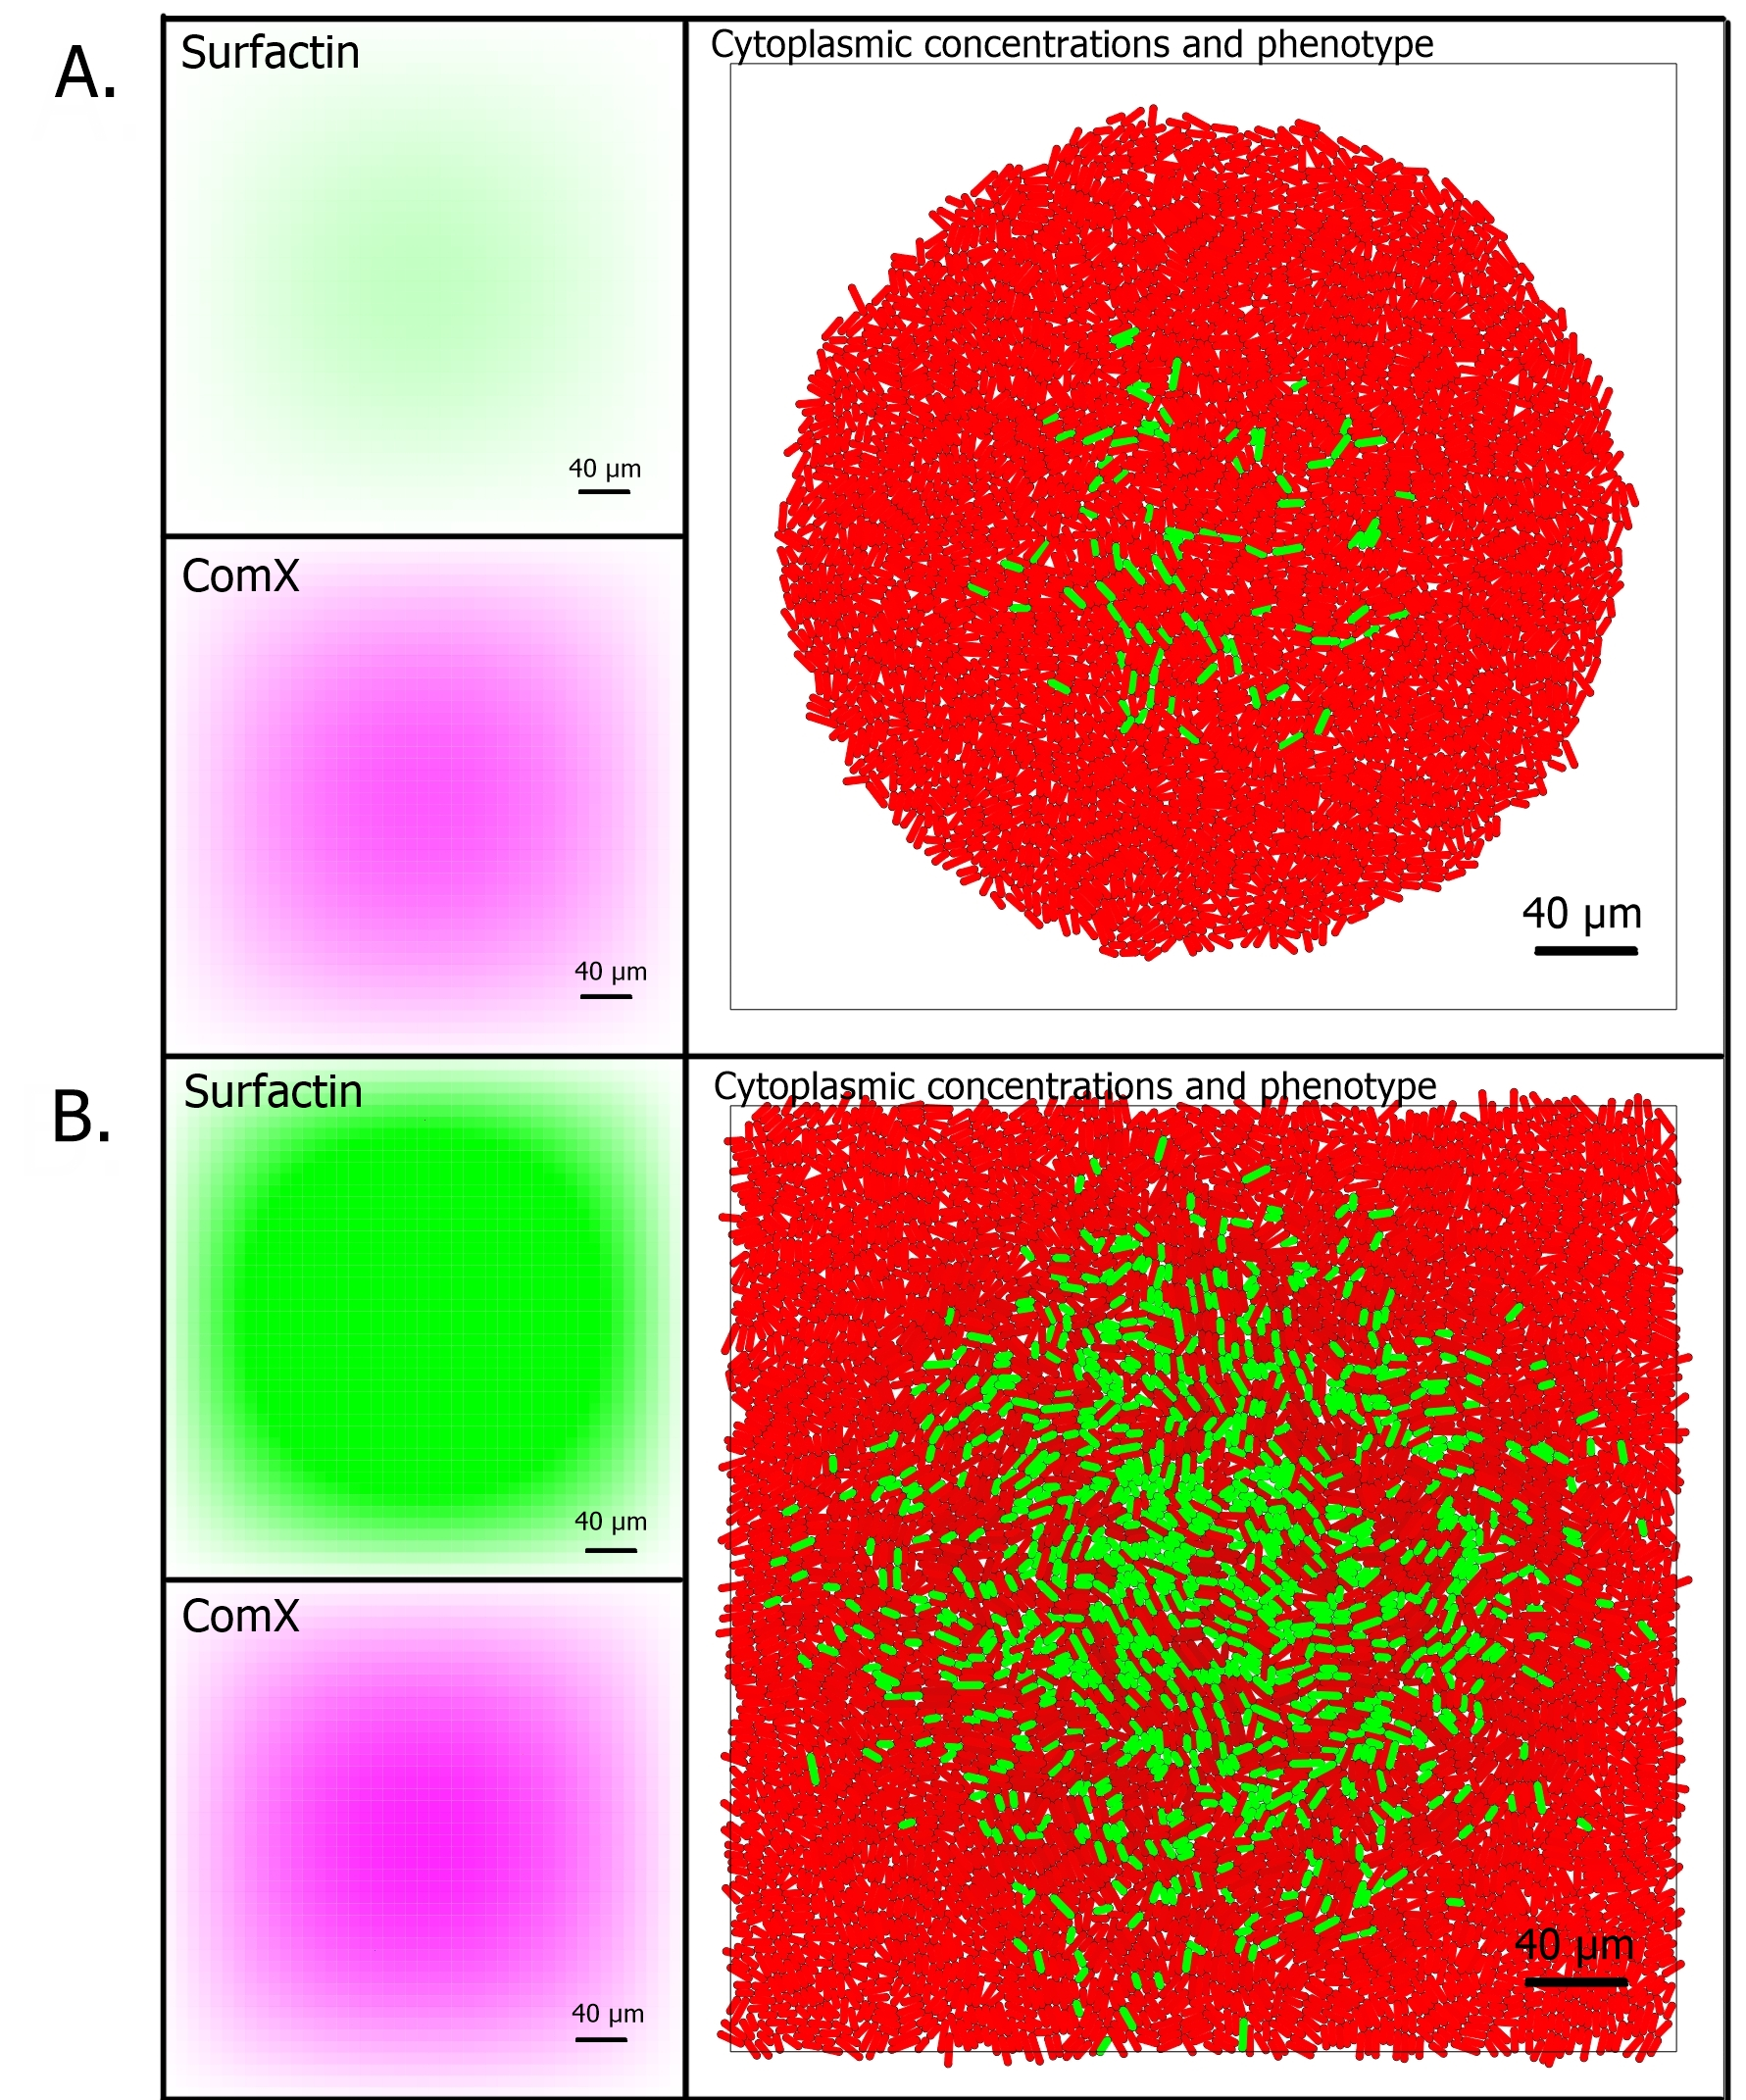
\includegraphics[width=0.98\textwidth]{Final_run2.jpg}
    \caption{\footnotesize \textbf{Extracellular and intracellular concentrations of signaling molecules and gene regulatory proteins 5 and 6 hours after inoculation.} A. Shows the simulation's state after 5 hours. B. Shows the simulation's state after 6 hours. The images in the top-left corners of A and B show the extracellular concentration of surfactin across the biofilm in green, measured in arbitrary units. The images in the bottom left corners of A and B show the extracellular concentration of ComX across the biofilm in pink, measured in arbitrary units. On the right side of A and B, the surfactin producers are shown in green. The intracellular concentrations of SinR, SinI, and SlrR of the non-surfactin-producing cells are represented as a point in the three-dimensional red-green-blue additive color space. Specifically, the SinR concentration is mapped to the red channel, SinI to the green channel, and SlrR to the blue channel. Since all cells have a high concentration of SinR and a low concentration of SinI and SlrR, they all appear almost 100\% red. }


\end{figure}

\subsection{After 5 and 6 Hours}\label{sec:contrib3:theme1}
As the cell population grows, the concentration of the ComX pheromone increases throughout the entire two-dimensional space, particularly in the central region of the biofilm. An elevated extracellular concentration of this pheromone triggers the expression of the surfactin-producing phenotype in cells that are particularly sensitive to ComX. At this stage, we can observe that a certain amount of surfactin has accumulated in the extracellular space. However, the concentration of surfactin is not high enough to cause any significant alteration in the bacterial cytoplasmic state. The total number of intracellular regulatory proteins remains almost unchanged compared to the concentration observed at the 4th hour (see Figure 5.2.A).

At the 6th hour, we observed a significant increase in the number of cells producing surfactin, as well as a rise in the concentration of extracellular surfactin (see Figure 5.2.B). If we observe carefully, we can also notice a slight decrease in the intensity of the red color in cells located at the center of the biofilm. This indicates a slight decrease in the concentration of SinR.


\begin{figure}[h]
    \centering
    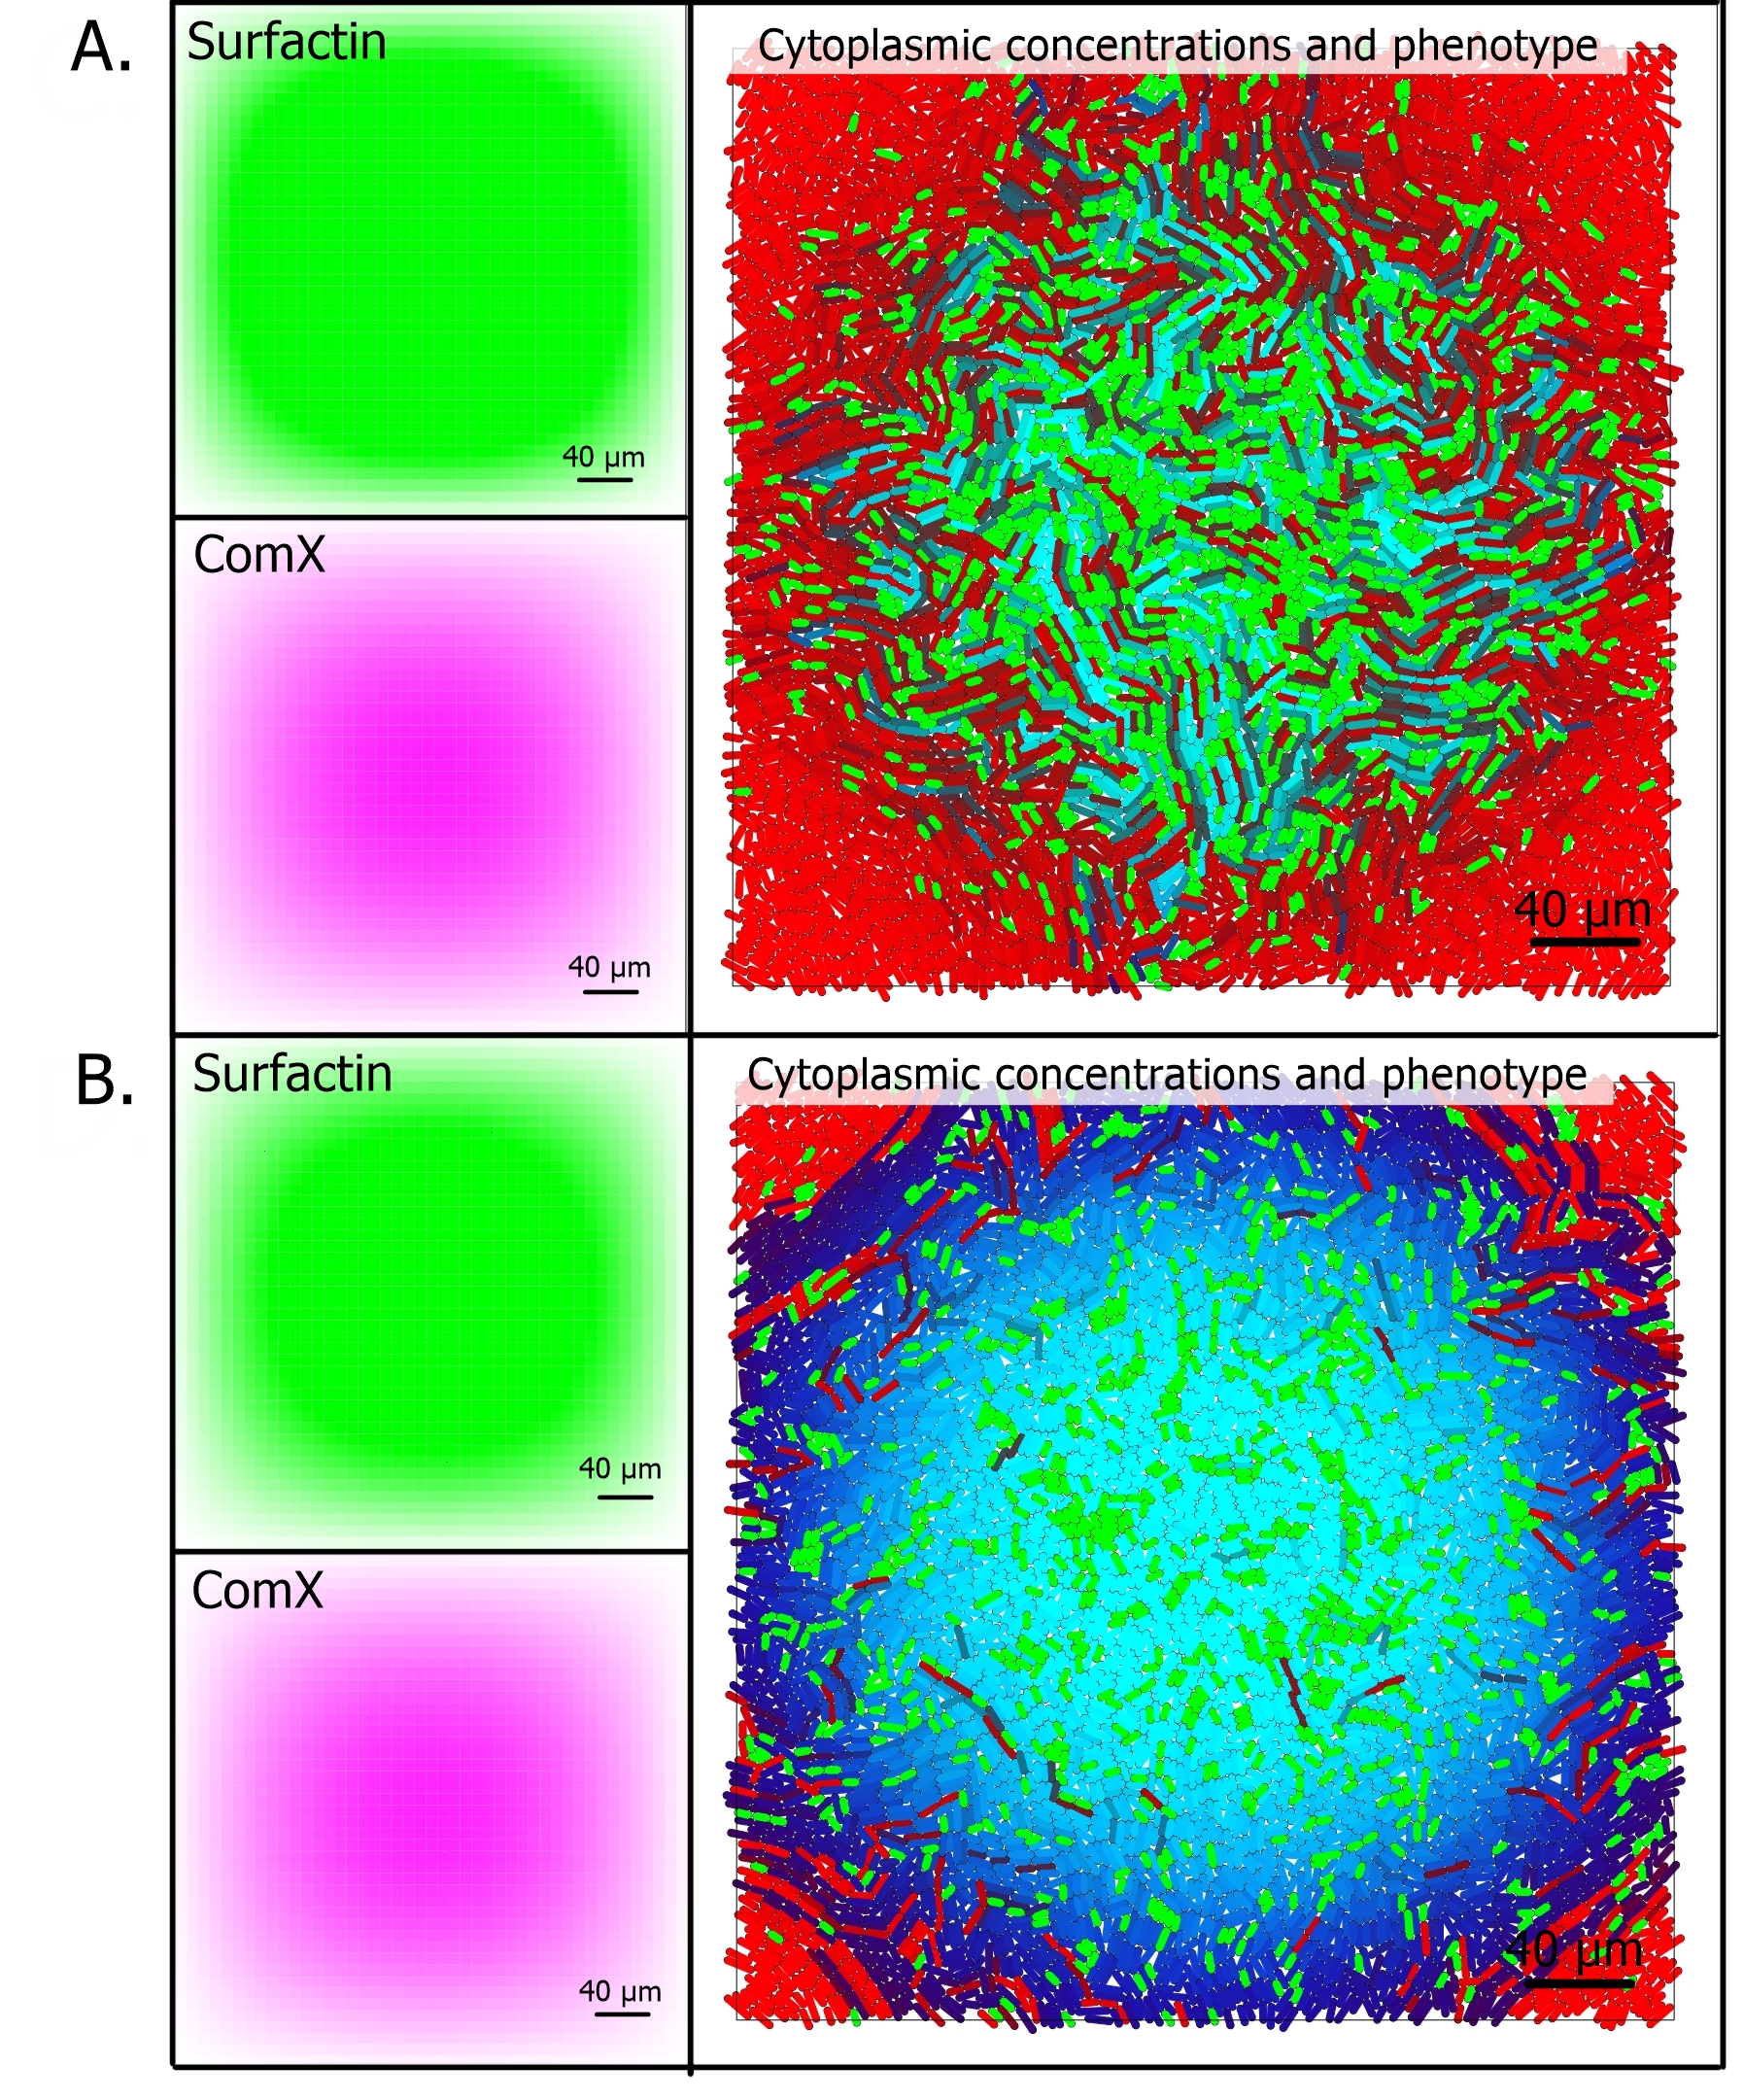
\includegraphics[width=0.98\textwidth]{Final_run3.jpg}
        \caption{\footnotesize \textbf{Extracellular and intracellular concentrations of signaling molecules and gene regulatory proteins 7 and 8 hours after inoculation.} A. Shows the simulation's state after 7 hours. B. Shows the simulation's state after 8 hours. The images in the top-left corners of A and B show the extracellular concentration of surfactin across the biofilm in green, measured in arbitrary units. The images in the bottom left corners of A and B show the extracellular concentration of ComX across the biofilm in pink, measured in arbitrary units. On the right side of A and B, the surfactin producers are shown in green. The intracellular concentrations of SinR, SinI, and SlrR of the non-surfactin-producing cells are represented as a point in the three-dimensional red-green-blue additive color space. Specifically, the SinR concentration is mapped to the red channel, SinI to the green channel, and SlrR to the blue channel. This way, cells with a high concentration of only SinR appear red. Cells with a high concentration of only SlrR appear blue. Cells with a high concentration of both SlrR and SinI appear in cyan. There are no cells that have only a high concentration of SinI.}

\end{figure}
\subsection{After 7 and 8 Hours}\label{sec:contrib3:theme1}

After 7 hours, a high concentration of surfactin activates the transcription of SinI, thereby increasing the concentration of SinI molecules in the cytoplasm. The SinI protein binds to SinR, forming a complex that effectively reduces the number of available SinR molecules in the cytoplasm. This is the reason for the significant decrease in the concentration of SinR in cells situated at the center of the biofilm. At the same time, we observe an increase in the concentration of SlrR, particularly in cells located near the center of the biofilm. This happens when the concentration of SinR drops below a threshold at which it becomes ineffective in inhibiting the expression of SlrR. (Figure 5.3.A)

At this stage, we can observe that many of the cells at the center of the biofilm have a very low concentration of SinR, which allows for the activation of the matrix production phenotype. This phenotype has the unique characteristic of being insensitive to ComX. This implies that as long as the bacteria continue to produce extracellular matrix, they will be unable to sense ComX and will not activate the surfactin-producing phenotype. In this scenario, if the majority of cells in the simulation are matrix producers and they continue to grow and reproduce, they will push the surfactin producers outside the simulation area. Over time, the biofilm will eventually displace its entire population of surfactin-producing cells, which are unable to grow and reproduce. (Figure 5.3.B)

As a result, a decrease in the concentration of surfactin will lead to a reduction in the production of SinI. Because of that, there will be an increase in the concentration of SinR, which will ultimately inhibit matrix production. The described phenomenon leads to oscillatory behavior in the composition of phenotypes. (Figures 5.5)

\begin{figure}[h]
    \centering
    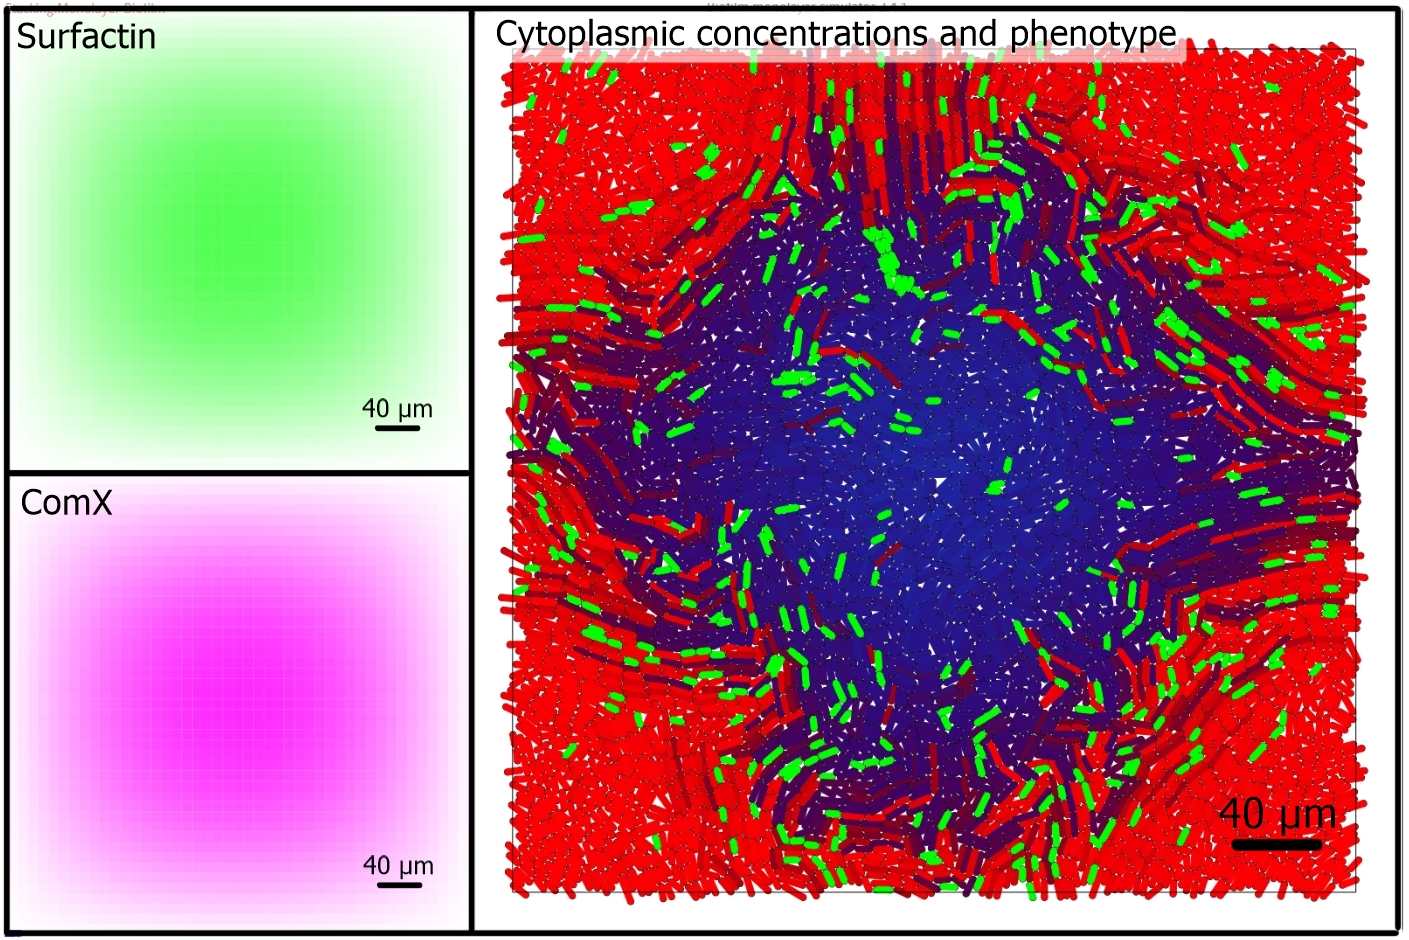
\includegraphics[width=0.98\textwidth]{elfin.jpg}
    \caption{\footnotesize \textbf{Extracellular and intracellular concentrations of signaling molecules and gene regulatory proteins 12 hours after inoculation.} The image in the top-left corner shows the extracellular concentration of surfactin across the biofilm in green, measured in arbitrary units. The image in the bottom left corner show the extracellular concentration of ComX across the biofilm in pink, measured in arbitrary units. On the right, the surfactin producers are shown in green. The intracellular concentrations of SinR, SinI, and SlrR of the non-surfactin-producing cells are represented as a point in the three-dimensional red-green-blue additive color space. Specifically, the SinR concentration is mapped to the red channel, SinI to the green channel, and SlrR to the blue channel. This way, cells with a high concentration of only SinR appear red. Cells with a high concentration of only SlrR appear in Blue. There are no cells that have only a high concentration of SinI.}



\end{figure}

\subsection{After 12 Hours}\label{sec:contrib3:theme1}

At this stage, we can observe that in many cells, the concentration of SinI and SlrR has decreased, while the concentration of SinR has increased, compared to the state after 8 hours. (See Figure 5.4). This indicates that the transition from high-SinR to low-SinR concentration is not permanent, but rather it continues to evolve as the concentration of surfactin decreases in the environment.


\clearpage

\section{Phenotype oscillations}
When plotting the number of cells exhibiting each phenotype, it becomes evident that the composition of phenotypes continues to oscilate as time increases.

In Figure 5.5, we can observe that the number of bacteria producing the matrix has reached its peak at approximately the 9th hour. At this time step, most cells are resistant to ComX due to the presence of the extracellular matrix. No matter how high the concentration of ComX is, it cannot activate the surfactin-producing phenotype in most cells. At the same time, undifferentiated cells and matrix-producing cells continue to grow and reproduce, displacing the few existing surfactin producers out of the simulation area. This causes a drop in surfactin producers at around the 10th hour. Upon examining the development of the biofilm within the first 20 hours (Figure 5.5), it becomes apparent that the composition of phenotypes continues to oscillate, showing no signs of equilibrium.

\begin{figure}[h]
    \centering
    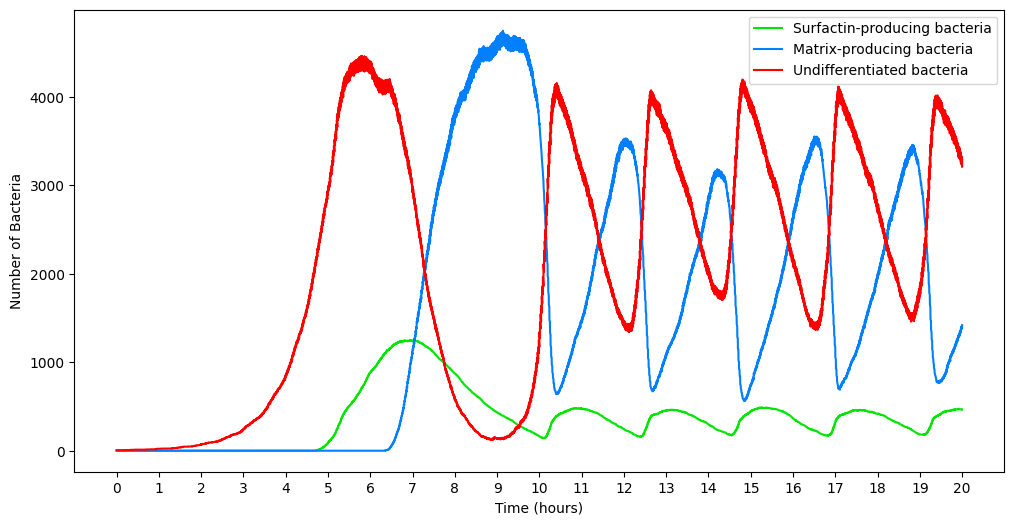
\includegraphics[width=1\textwidth]{phenotype_short.png}
    \caption{\footnotesize \textbf{Count of cell phenotypes throughout the simulation.} The quantities of matrix producers, surfactin producers, and undifferentiated cells are shown on the left axis. The maximum number of cells allowed at any given time is approximately 5200 bacteria.}


    
\end{figure} 

 



%\section{Minute 300th}\label{sec:contrib3:theme1}

%\begin{figure}[h]
  %  \centering
   % \includegraphics[width=1\textwidth]{300_minutes}
 %   \caption{\textbf{Extracellular and intracellular concentrations of signaling molecules and gene regulatory proteins 300 minutes after inoculation.} The top-left image in the diagram displays the color-coded cell phenotype, as well as the extracellular concentration of ComX. Cells with an undifferentiated phenotype are represented in pink, cells expressing the surfactin-producing phenotype are represented in green, and cells expressing the matrix producing phenotype are represented in blue. The extracellular ComX concentration is represented by a pink gradient in the background and is measured in arbitrary units. The images in the top-right, bottom-left, and bottom-right show the cytoplasmic counts of SinR, SinI, and SlrR molecules within individual cells. The scale ranges from black, indicating zero molecules, to white, indicating 85 or more molecules. These last three images also illustrate the concentration of extracellular surfactin, depicted as a green gradient in the background. The concentration of surfactin is measured in arbitrary units.}
    
%\end{figure}
\clearpage



\section{Conclusion}

In this chapter, we presented the sequential development of a simulated biofilm monolayer. We analyzed the evolution of the cytoplasmic proteins involved in the gene regulatory network and gave a detailed explanation and interpretation of the development of phenotypes. In the next chapter, we will present the conclusions of this thesis and discuss the future work and possible applications of the model.


\chapter{Conclusions and Future Work}\label{chap:conclusion}

\section{Summary of Outcomes}\label{sec:summary_Ch7}
This thesis represents a significant achievement in the field of computational biology by introducing a novel agent-based model that simulates the signaling pathways in \textit{Bacillus subtilis} involved in the initial phase of biofilm formation and matrix production. It is the first of its kind to integrate the dynamics of ComX and surfactin signaling, along with intracellular regulatory mechanisms involving the transcription factors SinI, SinR, and SlrR that respond to extracellular environmental conditions. Furthermore, the model accounts for volume exclusion interactions that occur due to physical constraints within the biofilm, as well as the processes of cell growth, reproduction, and the inheritance of cytoplasmic composition from one generation to the next. While there are existing models applied to \textit{B. subtilis} that address some aspects of biofilm behavior or intracellular processes in isolation, this work is unprecedented in its comprehensive approach that combines molecular, cellular, and intercellular scales to provide an in-depth understanding of biofilm formation in \textit{Bacillus subtilis}. The inclusion of such detailed biological details at multiple scales of magnitude has not been previously attempted in existing agent-based models of biofilm formation and matrix production in \textit{B. subtilis}, making this model unique among its peers. Additionally, the model exhibited behaviors in its simulations that are consistent with previously published results. This consistency underscores the model's value as a tool for evaluating the current understanding of signal pathways and gene regulation that drive the emergent behaviors observed in biofilms.

Furthermore, the model is designed with flexibility in mind, allowing for easy updates and modifications. This means that if future studies reveal new details about molecular mechanisms or the overall behavior of biofilms, the model can be easily adjusted to investigate how these new insights might impact the complex process of biofilm formation.

\section{Recommendations \& Future Work}\label{sec:future_Ch7}

\textbf{Accurate Physics Simulations}.

The significant computational power required to simulate volume exclusion interactions between cells limits the number of bacteria that can be simultaneously simulated. Furthermore, utilizing the library Box2d.ts to simulate the physical interactions of rigid objects may impose limitations on the types of mechanical simulations that can accurately model the volume exclusion forces between bacteria. One potential improvement of the model would be to integrate a scientific simulation library capable of accurately handling mechanical interactions between soft bodies and considering the semi-solid microscopic environment commonly found in biofilms.


\textbf{Simulation Parameters}.

In our efforts to create a simple yet accurate model, we made some significant assumptions that may potentially reduce the model's accuracy. For instance, the parameters used in Table 4.1 and the presumed protein concentration in the cytoplasm (SinI, SlrR, and SinR) are not based on direct experimental data. Instead, they are based on indirect calculations and computer simulations developed by other researchers. Additionally, the actual rate of secretion of signaling molecules was not taken into consideration. Instead, a dimensionless parameter was used to address the knowledge gap in this aspect of the signaling network. Finally, since the concentrations of these signaling molecules did not have any real units, the sensitivity to ComX and surfactin was also hypothesized.


\textbf{Adding Short-Range Quorum Sensing and Signal Molecule Uptake}.

The agent-based model presented in this thesis simulates long-range bacterial communication, which is an important factor in understanding the emergent properties of biofilms. However, a wealth of recent evidence, including findings reported in {\footnotesize\cite{vanGestel2021}}, suggests that understanding short-range interactions (where signaling molecules propagate no more than a few microns from the source due to irreversible cellular uptake) is essential for capturing the finer details of microbial communication. Consequently, future developments of the model should include provisions for short-range cell communication and the absorption of signaling molecules by neighboring cells. This additional level of detail would allow for a more precise simulation of the localized conditions that bacteria encounter.


\textbf{\textit{De novo} gene circuit design}.

In addition to being a useful tool for analyzing known genetic circuits and signaling networks in \textit{Bacillus subtilis}, we expect this model to be valuable for designing and testing \textit{de novo} gene circuits in a wide variety of bacterial species. To accomplish this, we would need to modify the equations described in section 2.4.3, the signaling molecules being secreted, and the rules that define the behavior of each phenotype (e.g., growth rate and sensitivity to chemical signals).

\textbf{Exploring Self-Healing Properties of Biofilms}.

Recent studies have revealed the ability of \textit{Bacillus subtilis} biofilms to self-repair after damage caused by physical cutting to the biofilm. This phenomenon, similar to wound healing, shows the resilience and adaptive capabilities of biofilms {\footnotesize\cite{Wang2021}\cite{Dong2022}\cite{Dong2022_1}}. The agent-based model developed in this thesis can be used as a tool to explore the mechanisms of this self-healing process. By simulating the signaling networks that facilitate communication among cells at the site of injury, this model has the potential to offer new insights into the coordinated cellular responses that drive biofilm recovery. By adjusting simulation conditions, it would be possible to recreate scenarios of biofilm damage and observe the subsequent biological processes that contribute to the biofilm's self-healing mechanism.


\chapter{Software Documentation}

% This is totally free-form - you can break it down by chapter, or integrate
% it. This is not at all critical.

% Set this up for MATLAB - you can tweak it for other languages. This could go in the toplevel preamble if you prefer.


\section{\texttt{Box2d} library}

\texttt{Box2D} is an open-source 2D physics engine used in game development. It manages the simulation of rigid bodies, handling collision detection, movement, and various physical properties like gravity and friction. Its performance and flexibility make it a popular choice among developers for adding realistic physics to games.

The original \texttt{Box2D} library was written in C++ by Erin Catto, and has since been ported to many other languages. The Github repository of the C++ version can be found at: \\ 
\url{https://github.com/erincatto/box2d.git}

The TypeScript version, \texttt{Box2D.ts}, was used in this thesis to simulate the physics volume exclusion interactions between cells.  The Github repository of the TypeScript version can be found at: \\ 
\url{https://github.com/flyover/box2d.ts.git}


\section{Biofilm Monolayer Simulatior}

The main code for the agent based model is written in TypeScript. The code is available at: \\
\url{https://github.com/CritalMediumBlue/box2d_for_bacteria.git}

The code has many unused example files inherited from the \texttt{Box2D.ts} library, these files are not relevant in this thesis but are kept for future reference. 
The relevant file used in this thesis is \texttt{pyramid.js}, which was originally an example file from the \texttt{Box2D.ts} library. This file was modified to simulate the physics of the biofilm monolayer. 


\section{Small Auxiliary repository}

The code for the auxiliary scripts used in this thesis is available at:\\

\url{https://github.com/CritalMediumBlue/ploter.git}

The repository contains the following folders:

\begin{itemize}
	\item \texttt{comparison} - Contains an HTML file showing two videos side by side. It was used for comparing the results of two physics engines (Box2D.ts and Matter.js) when simulating the biofilm monolayer.
	\item \texttt{plotter ode} - Contains an HTML file showing the 3D phase space with the solutions of system of ODEs used to model the gene regulatory network.
	\item \texttt{random plotter} - Contains an HTML file with a video that demonstrates an experiment with cells reproducing and inheriting the color of their parents with some random variations.
\end{itemize}
% Some examples of using the code - sample workflow



\printbibliography


% Optional; if you've written code, you want to include some basic
% documentation. Also include the git repository details if you have
% published the code.



\end{document}
